\chapter{Fast and Expressive Anonymous Credentials from New Rerandomizable Signatures}\label{chap2}
% \chapter{Fast and Expressive Anonymous Credentials from New Rerandomizable Signatures}\label{chap2}


\subsection{Motivation}

Digital interactions are shifting toward the self‑sovereign identity (SSI) model, where users control cryptographic credentials in digital wallets. In this paradigm, a wallet is not just a storage container, but a user-controlled agent for issuing, holding, and presenting zero-knowledge proofs of credentials across interoperable systems. Governments and industry are mandating digital wallets (e.g., EU Digital Wallet Regulation \cite{noauthor_regulation_2024}; 13 U.S. jurisdictions issuing mobile driver’s licenses \cite{aamva_jurisdiction_nodate}). Credential Oracles \cite{zhang_deco_2020, celi_distefano_2025} are "feeder services" that generate verifiable data attestations from different sources such as Web 2.0 credentials, bank data, or offline information.  The digital attestations are associated with a user's credential wallet and stored "within" the wallet. Commodity devices—from smartphones to IoT sensors—will sign outputs (photos, logs, transactions) with device keys (e.g., C2PA \cite{c2paorg_content_2024}), turning everyday interactions into verifiable claims. As AI-generated media and deepfakes proliferate, cryptographic provenance becomes critical, exponentially increasing the volume and heterogeneity of credentials that wallets must manage.


Previous deployments of Anonymous Credentials like IBM's Idemix \cite{camenisch_design_2002} and IRMA \cite{fischer-hubner_towards_2013} based on CL-Signatures \cite{camenisch_design_2002, cimato_signature_2003}, Hyperledger Fabric \cite{androulaki_hyperledger_2018} based on BBS+ \cite{hutchison_constant-size_2006}, Microsoft's U-Prove \cite{dunkelman_formal_2016} based on Brands' signatures \cite{brands_rethinking_2000}, were deployed in pilot programs \cite{dunkelman_formal_2016}, and proved that these systems were secure, private and feature-rich, but inefficient for widespread adoption. Their implementations were based on early constructions I label as "previous generation" and lacked efficient credential verification procedures required for the expected user experience needed for large-scale uptake, which we illustrate below.

% The performance comparison in Table \ref{tab:anon_creds_performance_old_gen_vs_new} demonstrates that newer anonymous credential schemes, such as BBS+2016 \cite{camenisch_anonymous_2016} and PS-UTT22 \cite{tomescu_utt_2022}, outperform older schemes like BBS+06 \cite{hutchison_constant-size_2006} and PS16 \cite{sako_short_2016} by shifting zero-knowledge proofs from the target group $(\mathbb{G}_T)$ to the source group ($\mathbb{G}_1)$\footnote{CL04 \cite{hutchison_signature_2004} is included in previous generation}. For 30 attributes, older schemes require computing over 3$\ell$, and 2$\ell$ $\G_T$ points respectively with Show and Verify times of 39.21 ms (BBS+06) and 32.78 ms (PS16). In comparison, newer schemes compute only in $\G_1$ and minimize pairings, achieving times of 5.72 ms and 5.38 ms—speedups of 6.85x and 6.09x, respectively. These improvements maintain full functionality, including selective disclosure and unlinkability, and rely on standard security assumptions, enhancing the practicality of anonymous credentials for digital identity systems.





\subsection{Problems and Scope}

The proliferation of credential types, sources, and volume reveals three gaps in existing schemes:

\begin{enumerate}
   \item \textbf{Scalability for wallet-centric architectures.} In the SSI model, wallets will accumulate potentially thousands of heterogeneous credentials (identity documents, transaction receipts, device-signed content, oracle attestations). Presentation must remain succinct even in scenarios where proof aggregation is possible.

    \item \textbf{Security against untrusted issuers.} The decentralized ecosystem includes credential oracles, device-embedded signers, and third-party attesters with varying security assumptions. User privacy (unlinkability, anonymity) must hold even when issuers collude or behave arbitrarily, protecting users from tracking by malicious ecosystem participants.

    \item \textbf{Expressive, efficient zero-knowledge proofs.} Users need to prove dynamic policies over attribute sets (e.g., "prove I'm over 18 AND in EU AND my device captured this photo today"). Achieving rich predicate support beyond simple possession proofs, without heavy SNARK primitives, is essential for mobile device feasibility.

\end{enumerate}

Solving these challenges requires a foundational understanding of how anonymous credentials evolved to address similar scalability and security concerns. While existing systems have made significant progress, none fully address the demands of the SSI wallet-centric ecosystem I've described. To build this next-generation system, we must first examine the architectural decisions and cryptographic innovations that brought us to this point.

Anonymous credentials are a fundamental building block for privacy-preserving digital identity, aligning perfectly with the SSI principle that users should prove attributes without revealing full identity. Since their first inception by Chaum \cite{chaum_untraceable_1981}, they have evolved from theoretical constructs to practical systems deployed in real-world applications such as U-Prove, Idemix, and PrivacyPass \cite{camenisch_design_2002, dunkelman_formal_2016}, but none have been designed explicitly for wallet-centric architectures managing thousands of heterogeneous credentials. 

Despite these advances, current ABC systems face critical gaps that prevent wide-scale deployment in the SSI ecosystem I've outlined.  Systems like SPS-EQ \cite{fuchsbauer_structure-preserving_2019, hanaoka_improved_2022} and ACT \cite{guo_anonymous_2023} achieve high efficiency but support only limited predicates, while approaches based on zkSNARKs enable rich expressiveness \cite{rosenberg_zk-creds_2022} but at computational cost. Furthermore, many anonymous credential systems assume honest issuers, leaving users vulnerable to privacy breaches from malicious credential providers, especially when issuers might be credential oracles.

This chapter develops the cryptographic foundations needed for credential wallets. I address each of the identified challenges through four key contributions that together enable efficient, secure, and expressive anonymous credentials at the scale demanded by the SSI ecosystem:

\begin{enumerate}
    \item \textbf{Complete Security Proofs for an efficient PS signature variant from UTT:} I provide formal security proofs that were only sketched in \cite{tomescu_utt_2022}:
    \begin{itemize}
        \item Position-binding vector commitments under SDLP in the Algebraic Group Model (Section \ref{sec:commitment})
        \item EUF-CMA security for rerandomizable signatures over commitments under PS-LRSW (Section \ref{sec:formal_treatment_utt_rerand_sig})
        \item Satisfaction of Anonymous Credential model \cite{fuchsbauer_structure-preserving_2019} security properties—correctness, unforgeability, and anonymity—for multi-show operations (Section \ref{sec:abc})
    \end{itemize}

    \item \textbf{Fastest Show+Verify Operations:} My construction achieves 10-16\% faster verification than UTT \cite{tomescu_utt_2022} and outperforms the most popular BBS+ variant \cite{camenisch_anonymous_2016} - I validate through comprehensive benchmarks \ref{fig:show_verify_utt_us}.

    \item \textbf{Malicious Issuer Security through Key Verification Protocols:} I formalize anonymity guarantees against malicious issuer via mandatory key verification (Section \ref{subsec:malicious_issuer_security_guarantee}), preventing deanonymization attacks through maliciously generated keys—a vulnerability that existing schemes do not address.

    \item \textbf{Empirical Validation of Schnorr Protocol Efficiency:} Comprehensive benchmarks \ref{fig:schnorr-benchmarks} reveal that Schnorr protocols achieve sublinear complexity for attribute proofs via multi-scalar multiplication, outperforming theoretical predictions and enabling almost constant-size expressive predicate evaluation.
\end{enumerate}

\subsubsection*{Chapter Roadmap}
Section \ref{chap2:preliminaries} establishes the background preliminaries, section \ref{sec:formal_treatment_utt_rerand_sig} provides the first complete security proofs for our rerandomizable signature scheme. Section \ref{chap2:extending_utt_construction} presents my key optimization: moving signatures from $\G_1$ to $\G_2$ for 10-16\% faster verification, plus malicious issuer protection through key verification. Section \ref{chap2:expressive_proofs} demonstrates how Sigma protocols achieve efficient predicate evaluation over complex policies. Section \ref{sec:abc} constructs my complete credential system with security proofs. Section \ref{sec:performance_evaluation} validates my approach through benchmarks, showing state-of-the-art performance with up to 83\% verification speedup.






\section{Preliminaries}\label{chap2:preliminaries}

\subsection{Assumptions}

\begin{definition}[Discrete Logarithm Assumption (DLP)]\label{dlp}
Let $\G$ be a cyclic group of prime order $p$ with generator $g$. The discrete logarithm assumption \cite{DBLP:journals/tit/DiffieH76} states that for any PPT adversary $\mathcal{A}$, there exists a negligible function $\negl$ such that:
$$\Pr\left[\begin{array}{l}
    x \sample \Z_p \\
    x' \sample \mathcal{A}(\G, p, g, g^x)
\end{array} : x = x'\right] \leq \negl(\lambda)$$
where $\lambda$ is the security parameter.
\end{definition}


\begin{definition}[Symmetric Discrete Logarithm Assumption (SDLP)]\label{sdlp}
The SDLP assumption first proved in \cite{hutchison_get_2010} states that for any PPT adversary $\mathcal{A}$, we say the SDLP assumption holds if there exists a negligible function $\negl$ such that:
$$\Pr\left[\begin{array}{l}
    \BG = (p, \G_1, \G_2, \G_T, e, g, \tilde{g}) \sample \BGGen(1^\lambda) \\
    x \sample \Z_p \\
    x' \sample \mathcal{A}(\BG, g^x, \tilde{g}^x)
\end{array} : x = x'\right] \leq \negl(\lambda)$$
where validity of input can be verified by checking $e(g, \tilde{g}^x) = e(g^x, \tilde{g})$.
\end{definition} 


\begin{definition}[Bilinear map]\label{bggroup}
Let $\G_1, \G_2$ and $\G_T$ be cyclic groups of prime order $p$ both in multiplicative notation. Let $g, \tilde{g}$ be generators of $\G_1$ and $\G_2$ respectively. We call $e$ a bilinear pairing or map $e : \G_1 \times \G_2 \to G_T$ if it is efficiently computable and the following properties hold
\begin{itemize}
    \item Bilinearity: $e(g^a, \tilde{g}^b) = e(g^b, \tilde{g}^a) = e(g,\tilde{g})^{ab}$ $\forall$ $a,b \in \Z_p$
    \item Non-degeneracy: $e(g,\tilde{g}) \neq 1_{\G_T}$ i.e., $e(g,\tilde{g})$ is the generator $\G_T$
\end{itemize}
We use Type-3 pairings, those without efficiently computable isomorphism between $\G_1 \to \G_2$ which are widely used in practice \cite{DBLP:journals/iacr/ChatterjeeM09}.
    
\end{definition}

\begin{definition}[Bilinear Group Generator]\label{bggenerator}
    A bilinear-group generator \cite{fuchsbauer_structure-preserving_2019} $\BGGen$ is a polynomial-time algorithm that takes a security parameter $1^\lambda$ and outputs a description of a bilinear group $\BG = (p, \G_1, \G_2, \G_T, e, g, \tilde{g}) \sample \BGGen(1^\lambda)$. $\G_1 = \langle g \rangle, \G_2 = \langle \tilde{g} \rangle $ and $\G_T$ of prime order $p$ and pairing $e : \G_1 \times \G_2 \to \G_T$.
\end{definition}

\begin{definition}[Type-3 PS-LRSW Assumption]\label{def:pslrsw}
The PS-LRSW assumption is based off the LRSW assumption \cite{goos_pseudonym_2000}, extended in \cite{sako_short_2016}. 
For any PPT adversary $\mathcal{A}$, we say the Type-3 PS-LRSW  assumption holds in the generic bilinear group model if there exists a negligible function $\negl$ such that:
$$\Pr\left[\begin{array}{l}
    \BG = (p, \G_1, \G_2, \G_T, e, g, \tilde{g}) \sample \BGGen(1^\lambda) \\
    x,y \sample \Z_p, X \gets g^x, \tilde{X} \gets \tilde{g}^x, \tilde{Y} \gets \tilde{g}^y \\
    (m^*, P_1, P_2) \sample \mathcal{A}^{\mathcal{O}_{x,y}}(\BG, X, \tilde{Y})
\end{array} : \begin{array}{l}
    m^* \notin Q \land P_1 \neq 1_{\G_1} \land \\
    e(P_1, \tilde{X} \cdot \tilde{Y}^{m^*}) = e(P_2, \tilde{g})
\end{array}\right] \leq \negl$$
where $Q$ is the set of queries made to $\mathcal{O}_{x,y}$ with access to $x,y$ is defined by:
\[
\text{Oracle }\mathcal{O}_{x,y}(m): \text{ Samples } h \sample \G_1, \text{ Returns the pair } P = (h, h^{x+my})
\]

\end{definition}






\subsection{Dual-Group Pedersen Commitments}\label{sec:commitment}
In this section, I introduce a specialized extension of Pedersen commitments that supports vector messages, rerandomizability, and position binding. My main contribution is a security proof in the Algebraic Group Model (AGM) that establishes position binding based on the Symmetric Discrete Logarithm Problem (SDLP).


\begin{definition}[Commitment Scheme]\label{def:commitmentscheme}
A Commitment scheme $\mathsf{Com}$, as denoted \cite{feigenbaum_non-interactive_1992} and expanded \cite{goos_rapid_1997} is a tuple of probabilistic polynomial-time algorithms $(\mathsf{Setup}, \mathsf{Commit}, \mathsf{Open})$ where:
\begin{itemize}
    \item $\mathsf{Setup}(1^\lambda) \rightarrow \mathsf{ck}$: is a probabilistic algorithm that takes as input a security parameter $\lambda$ and outputs a commitment key $\mathsf{ck}$. The message space $\mathcal{M}$ is implicitly defined by $\mathsf{ck}$.
    
    \item $\mathsf{Commit}(\mathsf{ck}, m) \rightarrow (\mathsf{cm}, r)$: is a probabilistic algorithm that takes as input the commitment key $\mathsf{ck}$ and a message $m \in \mathcal{M}$. It outputs a commitment $\mathsf{cm}$ and an opening value $r$.
    
    \item $\mathsf{Open}(\mathsf{ck}, \mathsf{cm}, m, r) \rightarrow b$: is a deterministic algorithm that takes as input the commitment key $\mathsf{ck}$, a commitment $\mathsf{cm}$, a message $m$, and an opening value $r$. It outputs a bit $b \in \{0,1\}$, where 1 indicates a valid opening and 0 indicates an invalid opening.
\end{itemize}
\end{definition}

\begin{definition}[Correctness]
A commitment scheme $(\mathsf{Setup}, \mathsf{Commit}, \mathsf{Open})$ is correct if for all $\lambda \in \mathbb{N}$, all commitment keys $\mathsf{ck} \in [\mathsf{Setup}(1^\lambda)]$, and all messages $m \in \mathcal{M}$:
$$\Pr[(\mathsf{cm}, r) \sample \mathsf{Commit}(\mathsf{ck}, m) : \mathsf{Open}(\mathsf{ck}, \mathsf{cm}, m, r) = 1] = 1.$$
\end{definition}

\begin{definition}[Hiding]
A commitment scheme $(\mathsf{Setup}, \mathsf{Commit}, \mathsf{Open})$ is hiding if for all PPT adversaries $\mathcal{A}$, there exists a negligible function $\negl$ such that:
$$\left|\Pr\left[\begin{array}{l}
    \mathsf{ck} \sample \mathsf{Setup}(1^\lambda) \\
    (m_0, m_1) \sample \mathcal{A}(\mathsf{ck}) \\
    b \sample \{0,1\} \\
    (\mathsf{cm}, r) \sample \mathsf{Commit}(\mathsf{ck}, m_b) \\
    b' \sample \mathcal{A}(\mathsf{ck}, \mathsf{cm})
\end{array} : b' = b\right] - \frac{1}{2}\right| \leq \negl(\lambda)$$
\end{definition}

\begin{definition}[Binding]
A commitment scheme $(\mathsf{Setup}, \mathsf{Commit}, \mathsf{Open})$ is binding if for all PPT adversaries $\mathcal{A}$, there exists a negligible function $\negl$ such that:
$$\Pr\left[\begin{array}{l}
    \mathsf{ck} \sample \mathsf{Setup}(1^\lambda) \\
    (\mathsf{cm}, m_0, m_1, r_0, r_1) \sample \mathcal{A}(\mathsf{ck})
\end{array} : \begin{array}{l}
    m_0 \neq m_1 \land \\
    \mathsf{Open}(\mathsf{ck}, \mathsf{cm}, m_0, r_0) = 1 \land \\
    \mathsf{Open}(\mathsf{ck}, \mathsf{cm}, m_1, r_1) = 1
\end{array}\right] \leq \negl(\lambda)$$
\end{definition}



\subsubsection{Dual-Group Construction for Vector of Messages}

I instantiate a rerandomizable commitment scheme to a vector of messages in the bilinear group setting as per the construction in \cite{tomescu_utt_2022} to enable efficient integration with the signature scheme. Let $\G_1, \G_2$ be cyclic groups of prime order $p$ with an efficient Type-3 pairing $e: \G_1 \times \G_2 \to \G_T$.

\begin{itemize}
    \item $\mathsf{Setup}(1^\lambda, 1^n) \to \mathsf{ck}$:
    Sample generators $(g, \tilde{g}) \sample \G_1 \times \G_2$.
    For $i \in [1,n]$: Sample $y_i \sample \Z_p$, compute $(g_i, \tilde{g}_i) \gets (g^{y_i}, \tilde{g}^{y_i})$.
    Return $\mathsf{ck} \gets (g, (g_1,\ldots,g_n), \tilde{g}, (\tilde{g}_1,\ldots,\tilde{g}_n))$.
    
    \item $\mathsf{Commit}(\mathsf{ck}, \attrs) \to (\mathsf{cm}, \widetilde{\mathsf{cm}}, r)$:
    Parse $\mathsf{ck}$ as $(g, (g_1,\ldots,g_n), \tilde{g}, (\tilde{g}_1,\ldots,\tilde{g}_n))$.
    Sample $r \sample \Z_p$.
    Compute $\mathsf{cm} \gets g^r \prod_{i=1}^n g_i^{m_i}$ and $\widetilde{\mathsf{cm}} \gets \tilde{g}^r \prod_{i=1}^n \tilde{g}_i^{m_i}$.
    Return $(\mathsf{cm}, \widetilde{\mathsf{cm}}, r)$.
    
    \item $\mathsf{Open}(\mathsf{ck}, (\mathsf{cm}, \widetilde{\mathsf{cm}}), \attrs, r) \to \{0,1\}$:
    Check if $\mathsf{cm} = g^r \prod_{i=1}^n g_i^{m_i}$ and $\widetilde{\mathsf{cm}} = \tilde{g}^r \prod_{i=1}^n \tilde{g}_i^{m_i}$.
    Additionally, verify $e(\mathsf{cm}, \tilde{g}) = e(g, \widetilde{\mathsf{cm}})$.
    Return 1 if all checks pass, 0 otherwise.
    
    \item $\mathsf{Rerand}(\mathsf{ck}, (\mathsf{cm}, \widetilde{\mathsf{cm}}), \Delta_r) \to ({\mathsf{cm}}', \widetilde{\mathsf{cm}}', r')$:
    Compute ${\mathsf{cm}}' \gets \mathsf{cm} \cdot g^{\Delta_r}$ and $\widetilde{\mathsf{cm}}' \gets \widetilde{\mathsf{cm}} \cdot \tilde{g}^{\Delta_r}$.
    Set $r' \gets r + \Delta_r$.
    Return $({\mathsf{cm}}', \widetilde{\mathsf{cm}}', r')$.
\end{itemize}

This construction preserves the message vector while updating the randomness, making rerandomized commitments computationally indistinguishable from fresh commitments to the same message.









\subsection{Rerandomizable Signature over Commitments}\label{sec:rerandsig_commitment}



\begin{definition}[Digital Signature Scheme]\label{def:signaturescheme}
A signature scheme $\mathsf{Sig}$ is a tuple of probabilistic polynomial-time algorithms $(\mathsf{KeyGen}, \mathsf{Sign}, \mathsf{Verify})$ where:

\begin{itemize}
    \item $\mathsf{KeyGen}(1^\lambda) \rightarrow (\mathsf{sk}, \mathsf{pk})$: is a probabilistic algorithm that takes as input a security parameter $\lambda$ and outputs a secret signing key $\mathsf{sk}$ and a public verification key $\mathsf{pk}$. The message space $\mathcal{M}$ is implicitly defined by $\mathsf{pk}$.
    
    \item $\mathsf{Sign}(\mathsf{sk}, m; r) \rightarrow \sigma$: is a probabilistic algorithm that takes as input the secret key $\mathsf{sk}$, a message $m \in \mathcal{M}$, and random coins $r$ sampled from the randomness space $\mathcal{R}$. It outputs a signature $\sigma$.
    
    \item $\mathsf{Verify}(\mathsf{pk}, m, \sigma) \rightarrow b$: is a deterministic algorithm that takes as input the public key $\mathsf{pk}$, a message $m \in \mathcal{M}$, and a signature $\sigma$. It outputs a bit $b \in \{0,1\}$, where 1 indicates acceptance and 0 indicates rejection.
\end{itemize}
\end{definition}

\begin{definition}[Correctness]
A signature scheme $(\mathsf{KeyGen}, \mathsf{Sign}, \mathsf{Verify})$ is correct if for all $k \in \mathbb{N}$, all key pairs $(\mathsf{sk}, \mathsf{pk}) \in [\mathsf{KeyGen}(1^k)]$ and all $m \in \mathcal{M}$ we have:

$$\Pr[\mathsf{Verify}(m, \mathsf{Sign}(m, \mathsf{sk}), \mathsf{pk}) = 1] = 1.$$
\end{definition}

\begin{definition}[EUF-CMA Security]\label{def:euf-cma}
A digital signature scheme $(\mathsf{KeyGen}, \mathsf{Sign}, \mathsf{Verify})$ is existentially unforgeable \cite{DBLP:journals/siamcomp/GoldwasserMR88} under adaptive chosen-message attacks if for all PPT algorithms $\mathcal{A}$, there exists a negligible function $\negl$ such that: 
$$\Pr\left[\begin{array}{l}
    (\mathsf{sk}, \mathsf{pk}) \sample \mathsf{KeyGen}(1^\lambda) \\
    (m^*, \sigma^*) \sample \mathcal{A}^{\mathcal{O}_{\mathsf{sk}}}(\mathsf{pk})
\end{array} : \begin{array}{l}
    m^* \notin Q \land \\
    \mathsf{Verify}(m^*, \sigma^*, \mathsf{pk}) = 1
\end{array}\right] \leq \negl$$
where $Q$ is the set of queries made to $\mathcal{O}_{\mathsf{sk}}$ with access to $\mathsf{sk}$ is defined by:
\[
\text{Oracle }\mathcal{O}_{\mathsf{sk}}(m): \text{ Returns } \sigma \gets \mathsf{Sign}(m, \mathsf{sk})
\]
\end{definition}




\begin{definition}[Rerandomizable Signature]\label{def:rerandomizablesignature}
A rerandomizable signature as discussed in \cite{sako_short_2016} scheme over commitments $\mathsf{RS}$ extends a standard signature scheme with the following interface:
\begin{itemize}
    \item $\mathsf{KeyGen}(1^\lambda, \mathsf{ck}) \rightarrow (\mathsf{sk}, \mathsf{pk})$: Takes security parameter $\lambda$ and commitment key $\mathsf{ck}$, outputs signing key $\mathsf{sk}$ and verification key $\mathsf{pk}$.
    
    \item $\mathsf{Sign}(\mathsf{sk}, \mathsf{cm}; u) \rightarrow \sigma$: Signs commitment $\mathsf{cm}$ using signing key $\mathsf{sk}$ and randomness $u$.
    
    \item $\mathsf{Rerand}(\mathsf{pk}, \sigma, \Delta_r, \Delta_u) \rightarrow \sigma'$: Creates a rerandomized signature $\sigma'$ from signature $\sigma$ using randomization values $\Delta_r, \Delta_u$.
    
    \item $\mathsf{Verify}(\mathsf{pk}, \mathsf{cm}, \sigma) \rightarrow \{0,1\}$: Verifies signature $\sigma$ on commitment $\mathsf{cm}$ using public key $\mathsf{pk}$.
\end{itemize}
\end{definition}

\begin{definition}[Correctness]\label{def:rerandomizable-signature-correctness}
A rerandomizable signature scheme over commitments satisfies correctness if for all security parameters $\lambda$, all key pairs $(\mathsf{sk}, \mathsf{pk}) \in [\mathsf{KeyGen}(1^\lambda, \mathsf{ck})]$, all messages $m \in \mathcal{M}$, all valid commitments $\mathsf{cm} = \mathsf{CM.Commit}(\mathsf{ck}, m, r)$, and all randomness values $u, \Delta_r, \Delta_u$:

\begin{enumerate}
    \item \textbf{Basic Verification}: $\mathsf{Verify}(\mathsf{pk}, \mathsf{cm}, \mathsf{Sign}(\mathsf{sk}, \mathsf{cm}; u)) = 1$
    
    \item \textbf{Rerandomization Consistency}: $\mathsf{Verify}(\mathsf{pk}, \mathsf{CM.Rerand}(\mathsf{ck}, \mathsf{cm}, \Delta_r), \mathsf{Rerand}(\mathsf{pk}, \sigma, \Delta_r, \Delta_u)) = 1$ where $\sigma = \mathsf{Sign}(\mathsf{sk}, \mathsf{cm}; u)$
    
    \item \textbf{Rerandomization Equivalence}: The distribution of $\mathsf{Rerand}(\mathsf{pk}, \mathsf{Sign}(\mathsf{sk}, \mathsf{cm}; u), \Delta_r, \Delta_u)$ is computationally indistinguishable from $\mathsf{Sign}(\mathsf{sk}, \mathsf{CM.Rerand}(\mathsf{ck}, \mathsf{cm}, \Delta_r); u+\Delta_u)$
\end{enumerate}
\end{definition}


\begin{definition}[EUF-CMA Commitment]\label{def:eufcma-commitment}
We extend the EUF-CMA property of \cite{DBLP:journals/siamcomp/GoldwasserMR88} to rerandomizable signatures and commitment schemes as the message. We note it's existentially unforgeable under adaptive chosen message (commitment) attacks if for all PPT adversaries $\mathcal{A}$, there exists a negligible function $\negl$ such that:
    \begin{align*}
        &\Pr\left[
            \begin{array}{l}
                \mathsf{BG} \gets \mathsf{BGGen}(1^{\secparam}), \\
                \mathsf{ck} \gets \mathsf{CM.KeyGen}(\mathsf{BG}), \\
                (\sk, \pk) \gets \mathsf{KeyGen}(\mathsf{BG}), \\
                (m^*, \cm^*, \sigma^*) \gets \mathcal{A}^{\mathsf{Sign}(\sk, \cdot)}(\pk) \\
                \end{array}
                \quad : \quad
                \begin{array}{l}
                \cm^* = \mathsf{CM.Com}(\mathsf{ck}, m^*, r^*) \land \\
                \mathsf{RS.Ver}(\pk, \sigma^*, m^*) = 1 \land \\
                \cm^* \notin Q_{\cm}
            \end{array}
        \right] \leq \negl
    \end{align*}
where $Q_{\cm}$ is the set of all commitments queried to the signing oracle
\end{definition}


\begin{definition}[Anonymity]\label{def:anonymity}
The standard definition for anonymity \cite{goos_efficient_2001} An anonymous credential system $\mathcal{AC} = (\mathsf{Setup}, \mathsf{KeyGen}, \mathsf{Issue}, \mathsf{Show}, \mathsf{Verify})$ provides \emph{anonymity} if for any probabilistic polynomial-time adversary $\mathcal{A}$, the advantage in the following game is negligible:

\begin{enumerate}
\item The challenger runs $\mathsf{pp} \leftarrow \mathsf{Setup}(1^\lambda)$ and $(pk, sk) \leftarrow \mathsf{KeyGen}(\mathsf{pp})$, giving $(\mathsf{pp}, pk)$ to $\mathcal{A}$.
\item $\mathcal{A}$ adaptively makes issuing and showing queries for various users and attributes.
\item $\mathcal{A}$ chooses two users $\mathsf{id}_0, \mathsf{id}_1$ and attribute sets $\mathsf{attr}_0, \mathsf{attr}_1$ such that $\mathsf{attr}_0, \mathsf{attr}_1$ satisfy the same predicate $\phi$.
\item The challenger flips a coin $b \leftarrow \{0,1\}$, issues a credential to user $\mathsf{id}_b$ with attributes $\mathsf{attr}_b$, and provides $\mathcal{A}$ with a proof $\pi$ that $\mathsf{attr}_b$ satisfies $\phi$.
\item $\mathcal{A}$ outputs a guess $b'$ and wins if $b' = b$.
\end{enumerate}

The anonymity advantage is: $\mathsf{Adv}^{\text{anon}}_{\mathcal{AC}}(\mathcal{A}) = |\Pr[b' = b] - 1/2|$

Anonymity ensures that credential presentations reveal no information about the user's identity beyond what is explicitly proven about their attributes.
\end{definition}







\subsection{Zero Knowledge Proof of Knowledge and Sigma-protocols}\label{def:zeroknowledgeproofofoknowledge}
We base our definitions of Zero Knowledge on the works in \cite{goldreich_foundations_2007, goldwasser_knowledge_1985, DBLP:conf/crypto/BellareG92}.
Zero Knowledge \cite{goldwasser_knowledge_1985} Proofs of Knowledge \cite{DBLP:conf/crypto/BellareG92} enable two entities, a Prover and Verifier, to interact; the Prover convinces the Verifier they know some secret without yielding any additional information apart from the statement. $\Sigma$ protocols are based on Schnorr's construction \cite{schnorr_efficient_1991} based on the hardness of the discrete log problem, where a prover proves knowledge of a hidden exponent. Schnorr's construction leverages computational zero knowledge, that is, they are secure against bounded adversaries. $\Sigma$ protocols are an extremely efficient instantiation of zero knowledge, are extremely versatile, and heavily used in modern privacy protocols due to their simplicity, efficiency, and ease of understanding. We begin by introducing notation and definitions for Zero Knowledge and continue to $\Sigma-$protocols below. Interactive zero-knowledge proofs can be made non-interactive via the Fiat-Shamir transformation \cite{odlyzko_how_1986}. We do not include this in our protocols as we focus on feasibility; however, careful implementation of the Fiat-Shamir transformation is required, as many implementations contain vulnerabilities. There are attempts to standardise both $\Sigma-$protocols and the use of the Fiat-Shamir transformation \cite{stephan_krenn_proposal_2021}. I use the notation from \cite{DBLP:conf/eurocrypt/CamenischM99}. 


We begin by establishing the foundational concepts of zero-knowledge proofs and sigma protocols, which form the basis for our constructions.

\subsubsection{Relations and Languages}

\begin{definition}[Relation]
\label{def:relation}
aLet $\mathcal{R}$ be a binary relation between an input string $x$ and a witness string $w$ as per \cite{DBLP:conf/crypto/BellareG92, feige_zero-knowledge_1988}:
$$\mathcal{R} \subseteq \{0,1\}^* \times \{0,1\}^*$$
For $(x,w) \in \mathcal{R}$, we require that the length of $w$ is at most $p(|x|)$ for some polynomial $p$. We call $w$ a witness for the instance $x$. The language associated with $\mathcal{R}$ is defined as:
$$L_\mathcal{R} = \{x : \exists w \text{ such that } (x,w) \in \mathcal{R}\}$$
\end{definition}

\subsubsection{Interactive Zero-Knowledge Proofs}

\begin{definition}[Interactive Zero-Knowledge Proof]
\label{def:zkproof}
An interactive protocol between a prover $\mathcal{P}$ and a verifier $\mathcal{V}$ is a zero-knowledge proof for relation $\mathcal{R}$ if it satisfies:

\begin{itemize}
    \item \textbf{Completeness}: For all $(x,w) \in \mathcal{R}$:
    $$\Pr[(\mathcal{P}(w), \mathcal{V})(x) = 1] \geq 1 - \negl(\lambda)$$
    
    \item \textbf{Soundness}: For any computationally bounded prover $\mathcal{P}^*$ and $x \notin L_\mathcal{R}$:
    $$\Pr[(\mathcal{P}^*, \mathcal{V})(x) = 1] \leq \negl(\lambda)$$
    
    \item \textbf{Zero-Knowledge}: There exists a probabilistic polynomial-time simulator $\mathcal{S}$ such that for all $(x,w) \in \mathcal{R}$ and any verifier $\mathcal{V}^*$:
    $$\{\text{VIEW}_{\mathcal{V}^*}(\mathcal{P}(w), \mathcal{V}^*)(x)\} \approx_c \{\mathcal{S}(x)\}$$
    where $\text{VIEW}_{\mathcal{V}^*}$ denotes the view of $\mathcal{V}^*$ in the interaction, and $\approx_c$ denotes computational indistinguishability as discussed \cite{goldwasser_probabilistic_1982}.
\end{itemize}
\end{definition}

\begin{remark}
When the zero-knowledge property holds only for the honest verifier, we call the protocol \emph{Honest Verifier Zero-Knowledge} (HVZK).
\end{remark}

\subsubsection{Proofs of Knowledge}

\begin{definition}[Proof of Knowledge]
\label{def:pok}
Let $\kappa: \{0,1\}^* \rightarrow [0,1]$ be the knowledge error function. An interactive protocol $(\mathcal{P}, \mathcal{V})$ is a proof of knowledge for relation $\mathcal{R}$ with knowledge error $\kappa$ if:

\begin{itemize}
    \item \textbf{Completeness}: For all $(x,w) \in \mathcal{R}$:
    $$\Pr[(\mathcal{P}(w), \mathcal{V})(x) = 1] = 1$$
    
    \item \textbf{Knowledge Soundness}: There exists a probabilistic polynomial-time knowledge extractor $\mathcal{E}$ such that for any prover $\mathcal{P}^*$, if $\epsilon(x)$ denotes the probability that $\mathcal{V}$ accepts on input $x$ when interacting with $\mathcal{P}^*$, then whenever $\epsilon(x) > \kappa(x)$:
    \begin{itemize}
        \item $\mathcal{E}$ with oracle access to $\mathcal{P}^*$ outputs $w$ such that $(x,w) \in \mathcal{R}$
        \item The expected running time of $\mathcal{E}$ is at most:
        $$\frac{|x|^c}{\epsilon(x) - \kappa(x)}$$
        for some constant $c$, where oracle queries count as one step.
    \end{itemize}
\end{itemize}
\end{definition}

\subsubsection{Sigma Protocols}

\begin{definition}[Sigma Protocol]
\label{def:sigma}
A sigma protocol for relation $\mathcal{R}$ is a three-move public-coin protocol of the following form:
\begin{enumerate}
    \item \textbf{Commitment}: $\mathcal{P}(x,w)$ sends commitment $a$
    \item \textbf{Challenge}: $\mathcal{V}$ sends random challenge $e \leftarrow \{0,1\}^t$
    \item \textbf{Response}: $\mathcal{P}$ sends response $z$
\end{enumerate}

The verifier accepts if and only if the verification predicate $\phi(x,a,e,z) = 1$. 
\end{definition}

A sigma protocol must satisfy the following three properties:

\begin{itemize}
    \item \textbf{Completeness}: If $\mathcal{P}$ and $\mathcal{V}$ follow the protocol on input $x$ with witness $w$ where $(x,w) \in \mathcal{R}$, then $\mathcal{V}$ always accepts.
    
    \item \textbf{Special Soundness}: From any $x$ and any two accepting transcripts $(a,e,z)$ and $(a,e',z')$ where:
    \begin{itemize}
        \item Both transcripts share the \emph{same} commitment $a$
        \item The challenges are \emph{different}: $e \neq e'$
    \end{itemize}
    one can efficiently compute $w$ such that $(x,w) \in \mathcal{R}$.
    
    \begin{remark}
    standard soundness states that a cheating prover can't succeed. Special soundness states that the extractor, given two accepting transcripts with the same commitment but different challenges can "rewind" the protocol to recover the witness. 
    \end{remark}
    
    \item \textbf{Special Honest Verifier Zero-Knowledge (SHVZK)}: There exists a polynomial-time simulator $\mathcal{S}$ that on input $(x,e)$ outputs $(a,e,z)$ with the same distribution as real protocol transcripts between honest $\mathcal{P}$ and $\mathcal{V}$ where $\mathcal{V}$'s challenge is $e$.
    
    \begin{remark}
    The distinction between standard HVZK and "special" HVZK:
    \begin{itemize}
        \item \textbf{Standard HVZK}: The simulator receives only the public input $x$ and may choose the challenge $e$ itself to produce a convincing transcript.
        \item \textbf{Special HVZK}: The simulator receives both the public input $x$ \emph{and} a pre-specified challenge $e$, yet must still produce a transcript $(a,e,z)$ indistinguishable from real executions.
    \end{itemize}
    The "special" capability is that the simulator can handle \emph{any} externally chosen challenge, not just ones it selects. This stronger property is used in e.g. Fiat-Shamir transformation, where challenges are determined by a hash function rather than chosen by the simulator.
    \end{remark}
\end{itemize}

\begin{theorem}
\label{thm:sigma-pok}
Any sigma protocol for relation $\mathcal{R}$ with challenge length $t$ is a proof of knowledge with knowledge error $2^{-t}$.
\end{theorem}


\paragraph{Zero-Knowledge Proof of Knowledge Notation}: We use the notation $\mathsf{PoK}$ to denote an interactive zero-knowledge proof of knowledge protocol based on $\Sigma-$protocol. Following the framework from~\cite{damgard_sigma_2010, DBLP:conf/eurocrypt/CamenischM99}, a $\mathsf{PoK}$ for relation $\mathcal{R}$ allows a prover to convince a verifier of the relation $\mathcal{R}$ specified \ref{def:relation} and as:

$$\pi \gets \mathsf{PoK}\{(\text{private inputs}) : \text{public relation}\}$$

\begin{itemize}
    \item $\pi$ is the resulting proof transcript
    \item The parentheses contain the \textbf{private inputs} (witnesses) known only to the prover  
    \item The colon separates private inputs from the \textbf{public relation} that must be satisfied
    \item All variables not in parentheses are assumed to be public
\end{itemize}

\begin{example}[Commitment Opening Proof] for our commitment scheme \ref{def:commitmentscheme}
$$\pircom \gets \mathsf{PoK}\{(m_1,\ldots,m_\ell, r): \cm = g^{r} \prod_{i=1}^\ell g_i^{m_i}\}$$

This represents a zero-knowledge proof of knowledge of the relation where:
\begin{itemize}
    \item \textbf{Private inputs}: The prover knows messages $(m_1,\ldots,m_\ell)$ and randomness $(r)$
    \item \textbf{Public relation}: These inputs satisfy the commitment equation $\cm' = g^{r } \prod_{i=1}^\ell g_i^{m_i}$
    \item \textbf{Public inputs}: The commitment $\cm$ and generators $g, g_1, \ldots, g_\ell$ are known to both parties
\end{itemize}
\end{example}























































\section{Formal Treatment for UTT's Rerandomizable Signature Over Commitments}\label{sec:formal_treatment_utt_rerand_sig}
I build upon the rerandomizable signature scheme over commitments introduced in UTT~\cite{tomescu_utt_2022}. This signature scheme enables the anonymous credential system to present signatures that are both unlinkable and unforgeable without revealing the underlying identity attributes. My main contribution is the first complete and tight security proof in the Algebraic Group Model that establishes $\EUFCMA$ security with minimal assumptions (noted that \cite{tomescu_utt_2022} presents a proof sketch).


\section{Security Analysis in the Algebraic Group Model}
\label{sec:agm-analysis}

We analyze our constructions in the Algebraic Group Model (AGM) \cite{shacham_algebraic_2018, hanaoka_pairing-free_2022}, where adversaries must provide algebraic representations for group elements they output.

\begin{definition}[Algebraic Adversary]
Let $\mathcal{A}$ be an adversary that receives group elements $(g_1, \ldots, g_n) \in \mathbb{G}^n$ 
as input. We say $\mathcal{A}$ is algebraic if, whenever it outputs a group element $h \in \mathbb{G}$, 
it also provides coefficients $(\alpha_1, \ldots, \alpha_n) \in \mathbb{Z}_p^n$ such that:
$$h = \prod_{i=1}^n g_i^{\alpha_i}$$
\end{definition}





\subsection{Example - Pedersen Commitments Binding in AGM}
We begin with an example of using the AGM to prove Pedersen Commitments \ref{def:commitmentscheme} are Binding. 


\begin{theorem}[Pedersen Commitments are Binding in AGM]
Let $\mathsf{CM}$ be the Pedersen commitment scheme with commitment key $\mathsf{ck} = (g, h)$ where $h = g^y$ for unknown $y$. For any algebraic adversary $\mathcal{A}$:
$$\Pr[\mathcal{A} \text{ breaks binding}] \leq \mathsf{Adv}^{\mathsf{DL}}_{\mathcal{B}}(\lambda)$$
\end{theorem}

\begin{proof}
We construct a reduction algorithm $\mathcal{B}$ that uses any binding-breaking algebraic adversary $\mathcal{A}$ to solve the discrete logarithm problem.

\textbf{Reduction $\mathcal{B}$:}
\begin{enumerate}
\item $\mathcal{B}$ receives a DL challenge $(g, h)$ where $h = g^y$ and $y$ is unknown
\item $\mathcal{B}$ sets $\mathsf{ck} = (g, h)$ and runs $\mathcal{A}(\mathsf{ck})$
\item $\mathcal{A}$ outputs a commitment $\mathsf{cm}$ and two distinct openings: $(m_0, r_0)$ and $(m_1, r_1)$ with $m_0 \neq m_1$ (breaking binding).
\end{enumerate}

\textbf{Algebraic Extraction:} Since $\mathcal{A}$ is algebraic and has received only the group elements $(g, h)$, when it outputs $\mathsf{cm}$, it must provide coefficients $(\alpha, \beta)$ such that:
$$\mathsf{cm} = g^\alpha \cdot h^\beta$$

\textbf{Analysis:} The binding property is broken when:
$$\mathsf{cm} = g^{m_0} h^{r_0} = g^{m_1} h^{r_1}$$

Combining with the algebraic representation and substituting $h = g^y$:
$$g^{\alpha + \beta y} = g^{m_0 + r_0 y} = g^{m_1 + r_1 y}$$

This yields the system:
$$\alpha + \beta y = m_0 + r_0 y = m_1 + r_1 y$$

From the equality $m_0 + r_0 y = m_1 + r_1 y$ and the fact that $m_0 \neq m_1$, we must have $r_0 \neq r_1$. Therefore:
$$y = \frac{m_1 - m_0}{r_0 - r_1}$$

\textbf{Output:} $\mathcal{B}$ computes and outputs $y$, successfully solving the discrete logarithm problem.
\end{proof}

The AGM allows the reduction to extract the algebraic representation of $\mathsf{cm}$, which, combined with the two openings, provides enough linear equations to solve for the discrete logarithm $y$. 









































































\subsection{Position Binding Pedersen Commitments for a Vector of Messages}

Building on the standard commitment scheme defined in Section \ref{def:commitmentscheme}, I prove a multi-message pedersen commitment to be position binding in a similar sense to vector commitments \cite{gorbunov_pointproofs_2020}. Position binding states that once a vector of messages $m_1, \ldots, m_i$ is committed, the order of the messages is set in place and cannot be changed. This is heavily used in Anonymous Credentials particularly with $\Sigma-$protocols that prove knowledge of certain exponents. The benefit in my protocols is that a credential is defined with messages in certain positions, for example, a credential with the identifier at position $0$ of the array. A user can then prove they have an identical identifier in another credential with the responses of a $\Sigma-$protocol. This enables a prover to prove the equality of the attribute without showing the attribute itself, just that an exponent at the same position in two different commitments is equal. This requires that the commitments are position binding. 


\begin{definition}[Position Binding]\label{def:position-binding}
A commitment scheme with message vectors in $\mathcal{M}^n$ is position binding if for all PPT adversaries $\mathcal{A}$, there exists a negligible function $\negl$ such that:
\[
    \Pr
    \left[
        \begin{array}{l}
        \mathsf{ck} \sample \mathsf{Setup}(1^\lambda, 1^n) \\
        (\mathsf{cm}, i, \attrs_0, \attrs_1, r_0, r_1) \sample \mathcal{A}(\mathsf{ck}) 
        \end{array}
        : \begin{array}{l}
            \mathsf{Open}(\mathsf{ck}, \mathsf{cm}, \attrs_0, r_0) = 1 \land \\
            \mathsf{Open}(\mathsf{ck}, \mathsf{cm}, \attrs_1, r_1) = 1 \land \\
            \attrs_0[i] \neq \attrs_1[i] \land \\
            \attrs_0[j] = \attrs_1[j] \; \forall j \neq i
          \end{array}
    \right] \leq \negl(\lambda)
\]
This ensures that an adversary cannot open a commitment to two different values at any single position while keeping other positions constant.
\end{definition}


\begin{definition}[Rerandomizability]
A commitment scheme $\mathsf{Com} = (\mathsf{Setup}, \mathsf{Commit}, \mathsf{Open})$ is rerandomizable if it includes an additional algorithm $\mathsf{Rerand}$ such that:

\begin{itemize}
\item $\mathsf{Rerand}(\mathsf{ck}, \mathsf{cm}, \Delta_r) \rightarrow (\mathsf{cm}', r')$: is a probabilistic algorithm that takes as input the commitment key $\mathsf{ck}$, a commitment $\mathsf{cm}$, and additional randomness $\Delta_r$. It outputs a new commitment $\mathsf{cm}'$ and updated opening value $r'$.
\end{itemize}

For all $\lambda \in \mathbb{N}$, all $\mathsf{ck} \in [\mathsf{Setup}(1^\lambda)]$, all $m \in \mathcal{M}$, all $(\mathsf{cm}, r) \in [\mathsf{Commit}(\mathsf{ck}, m)]$, and all $\Delta_r$:
$$\Pr[(\mathsf{cm}', r') \sample \mathsf{Rerand}(\mathsf{ck}, \mathsf{cm}, \Delta_r) : \mathsf{Open}(\mathsf{ck}, \mathsf{cm}', m, r') = 1] = 1.$$

Furthermore, the distribution of $\mathsf{cm}'$ should be computationally indistinguishable from a fresh commitment to the same message.
\end{definition}



\subsection{SDLP and Position Binding Security Analysis in the AGM}

The dual-group Pedersen commitment scheme \ref{def:commitmentscheme} satisfies the following properties:

\begin{itemize}
    \item \textbf{Perfect Hiding:} For any $\attrs \in \Z_p^n$, $\mathsf{Commit}(\mathsf{ck}, \attrs)$ outputs $(\mathsf{cm}, \widetilde{\mathsf{cm}}, r)$ where $\mathsf{cm} = g^r \prod_{i=1}^n g_i^{m_i}$ and $\widetilde{\mathsf{cm}} = \tilde{g}^r \prod_{i=1}^n \tilde{g}_i^{m_i}$. Since $r \sample \Z_p$ is uniform, $\mathsf{cm}$ and $\widetilde{\mathsf{cm}}$ are uniformly distributed in $\G_1$ and $\G_2$, revealing no information about $\attrs$.

    \item \textbf{Position Binding:} Under the SDLP assumption in the AGM, the scheme is position binding. The reduction \ref{thereom_position_binding} embeds an SDLP instance at a random position, using the adversary’s algebraic break to extract the solution with advantage scaled by $1/n$.

    \item \textbf{Rerandomizability:} The $\mathsf{Rerand}$ algorithm outputs $(\mathsf{cm}', \widetilde{\mathsf{cm}}', r') = (\mathsf{cm} \cdot g^{\Delta_r}, \widetilde{\mathsf{cm}} \cdot \tilde{g}^{\Delta_r}, r + \Delta_r)$, which is a valid commitment to the same $\attrs$. Since $\Delta_r \sample \Z_p$ is uniform, the distribution matches a fresh commitment, satisfying rerandomizability perfectly by construction.

    \item \textbf{Binding:} Position binding implies standard binding, as any break of standard binding (distinct $\attrs_0 \neq \attrs_1$) violates position binding at some position.
\end{itemize}

\begin{theorem}\label{thereom_position_binding}
In the Algebraic Group Model \ref{sec:agm-analysis}, if the Symmetric Discrete Logarithm Problem (SDLP)\ref{sdlp} is hard in the bilinear group $\BG = (\G_1, \G_2, \G_T, e, p, g, \tilde{g})$, then the commitment scheme satisfies position binding. For any algebraic PPT adversary $\mathcal{A}$ against position binding, there exists a PPT reduction $\mathcal{B}$ against SDLP such that:

$$\mathsf{Adv}^{\mathsf{pos\text{-}bind}}_{\mathcal{A}, \mathsf{Com}}(\lambda) \leq n \cdot \mathsf{Adv}^{\mathsf{SDLP}}_{\mathcal{B}, BG}(\lambda),$$

where $n$ is the message vector length.
\end{theorem}

\begin{proof}
We construct a reduction where an algorithm $\mathcal{B}$ solves the Symmetric Discrete Logarithm Problem (SDLP) by leveraging an algebraic adversary $\mathcal{A}$ that breaks the position binding property of the commitment scheme.

\begin{enumerate}
    \item \textbf{Setup: SDLP Challenger $\mathcal{C}$.} An external SDLP challenger provides $\mathcal{B}$ with an SDLP instance $(g^x, \tilde{g}^x) \in \G_1 \times \G_2$, where $g$ and $\tilde{g}$ are generators of groups $\G_1$ and $\G_2$ (respectively) of prime order $p$, and $x \sample \Z_p$ is a random, unknown exponent that $\mathcal{B}$ aims to compute.

    \item \textbf{Reduction Algorithm $\mathcal{B}$.} $\mathcal{B}$ takes the SDLP instance and constructs a commitment key $\mathsf{ck}$ to feed to $\mathcal{A}$ as follows:

        \begin{enumerate}
        \item \textbf{Choose a random position.} Sample $i^* \sample [1, n]$ uniformly at random, where $n$ is the number of positions in the commitment scheme. This $i^*$ is $\mathcal{B}$'s guess for where $\mathcal{A}$ will break position binding.
        
        \item \textbf{Construct the commitment key $\mathsf{ck}$.}
        \begin{itemize}
            \item For position $i^*$, embed the SDLP instance: 
            $$(g_{i^*}, \tilde{g}_{i^*}) = (g^x, \tilde{g}^x).$$
            \item For all other positions $j \neq i^*$: Sample $y_j \sample \Z_p$ independently, set $(g_j, \tilde{g}_j) = (g^{y_j}, \tilde{g}^{y_j})$.
            \item Output $\mathsf{ck} = (g, (g_1, \ldots, g_n), \tilde{g}, (\tilde{g}_1, \ldots, \tilde{g}_n))$.
        \end{itemize}
        
        \item \textbf{Invoke the adversary.} $\mathcal{B}$ Runs $\mathcal{A}$ with input $\mathsf{ck}$: 
        $$\mathcal{A}(\mathsf{ck}) \rightarrow (\mathsf{cm}, \widetilde{\mathsf{cm}}, i, \attrs_0, \attrs_1, r_0, r_1).$$
        Here, $\mathcal{A}$ outputs a position binding break at position $i$, meaning $\attrs_0[i] \neq \attrs_1[i]$, and $\attrs_0[j] = \attrs_1[j]$ for all $j \neq i$, with $\mathsf{cm}$ opening to both $(\attrs_0, r_0)$ and $(\attrs_1, r_1)$.
    \end{enumerate}

    
      \item  \textbf{Adversary $\mathcal{A}$.} Since $\mathcal{A}$ is algebraic, it provides explicit representations of its outputs:
        \begin{itemize}
            \item For $\mathsf{cm} \in \G_1$: 
            $$\mathsf{cm} = g^{\alpha} \prod_{k=1}^n g_k^{\beta_k}$$
            where $\alpha, \beta_1, \ldots, \beta_n \in \Z_p$ are known to $\mathcal{B}$.
            \item For $\widetilde{\mathsf{cm}} \in \G_2$: 
            $$\widetilde{\mathsf{cm}} = \tilde{g}^{\tilde{\alpha}} \prod_{k=1}^n \tilde{g}_k^{\tilde{\beta}_k}$$
            where $\tilde{\alpha}, \tilde{\beta}_1, \ldots, \tilde{\beta}_n \in \Z_p$ are known to $\mathcal{B}$.
        \end{itemize}
        The opening conditions hold:
        \begin{itemize}
            \item $\mathsf{cm} = g^{r_0} \prod_{k=1}^n g_k^{m_{0,k}} = g^{r_1} \prod_{k=1}^n g_k^{m_{1,k}}$
            \item $\widetilde{\mathsf{cm}} = \tilde{g}^{r_0} \prod_{k=1}^n \tilde{g}_k^{m_{0,k}} = \tilde{g}^{r_1} \prod_{k=1}^n \tilde{g}_k^{m_{1,k}}$
            \item $e(\mathsf{cm}, \tilde{g}) = e(g, \widetilde{\mathsf{cm}})$.
        \end{itemize}


\textbf{Extraction by $\mathcal{B}$.} $\mathcal{B}$ uses $\mathcal{A}$'s output to solve for $x$:

\begin{enumerate}
        \item \textbf{Check the position.} If $i \neq i^*$, abort. If $i = i^*$, proceed.
        
        \item \textbf{Substitute generators and equate exponents.} Substitute into $\mathsf{cm}$: $g_k = g^{y_k}$ for $k \neq i^*$, and $g_{i^*} = g^x$. From the opening condition:
        $$\mathsf{cm} = g^{r_0} \prod_{k=1}^n g_k^{m_{0,k}} = g^{r_0} \cdot \prod_{k \neq i^*} g^{y_k m_{0,k}} \cdot g^{x m_{0,i^*}},$$
        and similarly:
        $$\mathsf{cm} = g^{r_1} \cdot \prod_{k \neq i^*} g^{y_k m_{1,k}} \cdot g^{x m_{1,i^*}}.$$
        Equate the exponents of $g$:
        $$r_0 + \sum_{k \neq i^*} y_k m_{0,k} + x m_{0,i^*} = r_1 + \sum_{k \neq i^*} y_k m_{1,k} + x m_{1,i^*}.$$
        
        \item \textbf{Simplify the equation.} Since $\attrs_0[j] = \attrs_1[j]$ for $j \neq i$, we have $m_{0,k} = m_{1,k}$ for all $k \neq i^*$. Cancel these terms:
        $$r_0 + x m_{0,i^*} = r_1 + x m_{1,i^*}.$$
        Rearrange:
        $$x (m_{0,i^*} - m_{1,i^*}) = r_1 - r_0.$$
        
        \item \textbf{Solve for $x$.} Since $i = i^*$ and $\attrs_0[i^*] \neq \attrs_1[i^*]$, it follows that $m_{0,i^*} \neq m_{1,i^*}$. Thus:
        $$x = \frac{r_1 - r_0}{m_{0,i^*} - m_{1,i^*}} \mod p.$$
        Output $x$ as the solution to the SDLP instance.
    \end{enumerate}

    \textbf{Success Probability.} $\mathcal{B}$ succeeds when $i = i^*$, which occurs with probability $1/n$. If $\mathcal{A}$ breaks position binding with probability $\epsilon$, then $\mathcal{B}$ solves SDLP with probability $\epsilon / n$.

\textbf{Pairing Check.} The condition $e(\mathsf{cm}, \tilde{g}) = e(g, \widetilde{\mathsf{cm}})$ ensures consistency across $\G_1$ and $\G_2$, but $\mathcal{B}$ relies solely on the $\G_1$ equations for extraction.
\end{enumerate}
\end{proof}





% We analyze the reduction's properties in detail:
% \begin{itemize}
%     \item \textbf{Perfect Simulation:} The commitment key distribution is identical to the real scheme:
%         \begin{itemize}
%             \item At position $i^*$: $(g_{i^*}, \tilde{g}_{i^*}) = (g^x, \tilde{g}^x)$ is uniformly distributed in $\G_1 \times \G_2$ by the SDLP instance properties
%             \item At positions $j \neq i^*$: $(g_j, \tilde{g}_j) = (g^{y_j}, \tilde{g}^{y_j})$ is uniform due to $y_j \sample \Z_p$
%             \item Therefore, from $\mathcal{A}$'s view, $\mathsf{ck}$ is distributed identically to the real scheme
%         \end{itemize}
    
%     \item \textbf{Extraction Success:} $\mathcal{B}$ successfully extracts the SDLP solution when:
%         \begin{itemize}
%             \item $\mathcal{A}$ outputs a valid position binding break (occurs with probability $\epsilon$)
%             \item The guessed position matches: $i = i^*$ (occurs with probability $1/\ell$)
%             \item The extraction equation is solvable: $m_{0,i^*} \neq m_{1,i^*}$ (guaranteed by definition of position binding break)
%         \end{itemize}
    
%     \item \textbf{Advantage Analysis:} Combining these probabilities:
%         \begin{itemize}
%             \item Events are independent as $i^*$ is chosen before $\mathcal{A}$'s execution
%             \item $\mathsf{Pr}[\mathcal{B} \text{ succeeds}] = \epsilon \cdot \frac{1}{\ell}$
%             \item Therefore: $\mathsf{Adv}^{\mathsf{SDLP}}_{\mathcal{B},\G}(\lambda) \geq \frac{1}{\ell} \cdot \mathsf{Adv}^{\mathsf{pos\text{-}bind}}_{\mathcal{A},\mathsf{RVC}}(\lambda)$
%         \end{itemize}
% \end{itemize}













\subsection{EUF-CMA Rerandomizable Signature over Commitments}\label{sig-construction}
We assume the existence of a commitment key $\ck$ from $\mathsf{CM.Setup}$ as input into the rerandomizable signature scheme $\mathsf{RS}$. We copy the algorithm below for convenience.
\begin{itemize}
    \item $\mathsf{CM.Setup}(\secparam, \ell, (y_i, \ldots, y_{\ell} \in \Z_p^{\ell})) \to \ck:$  
    Sample $(g, \tilde{g}) \sample \G_1 \times \G_2$, For $i \in [1,\ell]$: Compute $g_i = g^{y_i}$ and $\tilde{g}_i = \tilde{g}^{y_i}$. Return $\ck \gets (g, (g_1,\ldots,g_\ell), \tilde{g}, (\tilde{g}_1,\ldots,\tilde{g}_\ell))$
    
    \item $\mathsf{RS.KeyGen}(\secparam, \ck) \to (\sk, \vk):$ 
        Retrieve $(g, \cdot, \tilde{g}, \cdot)$ from $\mathsf{ck}$,
        Sample $x \sample \Z_p$,
        Set $(\sk, \vk) \gets (g^x, \tilde{g}^x)$, return $(\sk, \vk))$
        % Return $(\mathsf{sk} = (x,g), \mathsf{pk} = (\mathsf{pp}, \mathsf{vk}, \mathsf{ck}))$
    
    \item $\mathsf{RS.Sign}(\mathsf{sk}, \mathsf{cm}; u) \to \sigma:$ 
        Let $h \gets g^u$
        Return $\sigma \gets (h, (\sk \cdot \mathsf{cm})^u)$
    
    \item $\mathsf{RS.Rerand}(\sigma, \Delta_r, \Delta_u) \to \sigma':$
        Parse $\sigma$ as $(\sigma_1, \sigma_2)$
        Set $\sigma_1' \gets \sigma_1^{\Delta_u}$
        Set $\sigma_2' \gets (\sigma_2 \cdot \sigma_1^{\Delta_r})^{\Delta_u}$
        Return $\sigma' \gets (\sigma_1', \sigma_2')$
    
    \item $\mathsf{RS.Ver}(\vk, \cm, \sigma) \to \bit:$
        Parse $\sigma$ as $(\sigma_1, \sigma_2)$, The prover $\Prover$ runs a Proof of Knowledge protocol with the following relation 
    \[
        \mathcal{R} \gets \mathsf{PoK}\{(m_1,\ldots,m_\ell, r + \Delta_r): 
    \]
    \[
         e(\sigma_2', \tilde{g}) = e(\sigma_1', \vk)\cdot e(\sigma_1', \widetilde{\cm}') \quad \wedge \quad
        e(\cm', \tilde{g}) = e(g, \widetilde{\cm}') \quad \wedge \quad
        \cm' = g^{r + \Delta_r} \prod_{i=1}^\ell g_i^{m_i}
        \}
    \]
        
\end{itemize}






\subsection{Security Analysis in the AGM}

\begin{theorem}
The rerandomizable signature scheme is correct as defined \ref{def:rerandomizable-signature-correctness}.
\end{theorem}


\begin{proof}
First we demonstrate the prover's rerandomized signature verifies with the verification key $\mathsf{vk}$ and the rerandomized commitment. Essentially, we need the following pairing to hold for a valid signature verification:
\[
    e(\sigma_2', \tilde{g}) = e(\sigma_1', \mathsf{vk} \cdot \widetilde{\mathsf{cm}'})
\]

We manipulate the bilinearity properties \ref{bggroup} of the pairing groups to verify this equation:
    
\begin{align*}
    e(\sigma_2', \tilde{g}) &= e((\mathsf{sk} \cdot \mathsf{cm})^{u \cdot \Delta_u} \cdot h^{\Delta_u \cdot \Delta_r}, \tilde{g}) \\
    &= e(h^{x \cdot \Delta_u} \cdot \mathsf{cm}^{u \cdot \Delta_u} \cdot h^{\Delta_u \cdot \Delta_r}, \tilde{g}) \\
    &= e(h^{x \cdot \Delta_u}, \tilde{g}) \cdot e(\mathsf{cm}^{u \cdot \Delta_u}, \tilde{g}) \cdot e(h^{\Delta_u \cdot \Delta_r}, \tilde{g}) \\
    &= e(h^{\Delta_u}, \tilde{g}^x) \cdot e(\mathsf{cm}, \tilde{g})^{u \cdot \Delta_u} \cdot e(h^{\Delta_u}, \tilde{g})^{\Delta_r} \\
    &= e(\sigma_1', \mathsf{vk}) \cdot e(g^{u \cdot \Delta_u}, \widetilde{\mathsf{cm}}) \cdot e(\sigma_1', \tilde{g})^{\Delta_r} \\
    &= e(\sigma_1', \mathsf{vk}) \cdot e(\sigma_1', \widetilde{\mathsf{cm}}) \cdot e(\sigma_1', \tilde{g}^{\Delta_r}) \\
    &= e(\sigma_1', \mathsf{vk} \cdot \widetilde{\mathsf{cm}} \cdot \tilde{g}^{\Delta_r}) \\
    &= e(\sigma_1', \mathsf{vk} \cdot \widetilde{\mathsf{cm}'}) \\
\end{align*}
\end{proof}

Secondly, we need to verify knowledge of messages within the commitment. The Prover used $\widetilde{\mathsf{cm}'} \in \G_2$ during verification, which would be the natural method for a sigma-style proof of knowledge protocol, proving knowledge of the attributes of the commitment with $\G_2$ bases. However, due to the properties of the symmetric bilinear commitment \ref{sdlp}, we can prove the equality of $\mathsf{cm}' \in \G_1$ and $\widetilde{\mathsf{cm}'} \in \G_2$ to reduce $\G_2$ computation on both the prover and verifier during verification. 
Thus the prover computes the following to prove equality of commitments across groups:
\[
    e(\mathsf{cm}', \tilde{g}) = e(g, \widetilde{\mathsf{cm}}')
\]
Then proves the opening of the commitment in zero knowledge:
\[
 \pircom  \gets \mathsf{PoK}\{(m_1,\ldots,m_\ell, r + \Delta_r): \cm' = g^{r + \Delta_r} \prod_{i=1}^\ell g_i^{m_i}\}
\]






\begin{theorem}[EUF-CMA Security]
Assume the PS-LRSW \ref{def:pslrsw} assumption holds and the Pedersen commitment is computationally binding. Then, in the Algebraic Group Model \ref{sec:agm-analysis}, the rerandomizable signature scheme is existentially unforgeable under adaptive chosen-message(commitment) attacks \ref{def:eufcma-commitment}. For any algebraic PPT adversary $\mathcal{A}$, there exist PPT reductions $\mathcal{B}_0, \mathcal{B}_1$ such that:
\[
\Adv^{\mathsf{EUF\mbox{-}CMA}}_{\mathsf{RS},\mathcal{A}}(\lambda) \leq \Adv^{\mathsf{PS\mbox{-}LRSW}}_{\mathcal{B}_0}(\lambda) + \Adv^{\mathsf{Binding}}_{\mathcal{B}_1}(\lambda) + \frac{q_v + q_s}{p},
\]
where $q_v$ (verification) and $q_s$ (signing) are query counts.
\end{theorem}

\begin{proof}\label{eufcma-proof}
We construct two reductions handling different forgery types. Let $\mathcal{A}$ be an adversary with advantage $\epsilon$.

\textbf{Reduction Strategy: } Since we don't know in advance which type of forgery $\AdvA$ will produce, we design two reductions:
\begin{itemize}
    \item $\mathcal{B}_0$ handles forgeries with a new message combination
    \item $\mathcal{B}_1$ handles forgeries where the same message appears in different commitments
\end{itemize}

\paragraph{1. Setup}
Given a PS-LRSW challenge $(g, \tilde{g}, X=g^x, \tilde{X}=\tilde{g}^x, Y=g^y, \tilde{Y}=\tilde{g}^y)$, both reductions:
\begin{itemize}
    \item Sample $\alpha_1, \alpha_2, \beta_1, \beta_2 \sample \Z_p$ 
    \item Set commitment base elements $g_i = Y^{\alpha_i}g^{\beta_i}$ and $\tilde{g}_i = \tilde{Y}^{\alpha_i}\tilde{g}^{\beta_i}$ for $i \in \{1,2\}$
    \item Set $\mathsf{pk} = (\tilde{X}, \mathsf{ck} = (g, g_1, g_2, \tilde{g}, \tilde{g}_1, \tilde{g}_2))$
    \item Send $\mathsf{pk}$ to $\mathcal{A}$
\end{itemize}

\paragraph{2. Oracle Simulation}
For a signing query on commitment $\mathsf{cm} = g_1^{m_1}g_2^{m_2}g^r$:
\begin{itemize}
    \item $\mathcal{B}_0$ (PS-LRSW Reduction):
    \begin{enumerate}
        \item Compute $m = \alpha_1m_1 + \alpha_2m_2$ 
        \item Query PS-LRSW oracle to get $(h, h^{x+my})$
        \item Return $\sigma = (h, h^{x+my} \cdot h^{\beta_1m_1 + \beta_2m_2 + r})$
    \end{enumerate}
    
    \item $\mathcal{B}_1$ (Binding Reduction):
    \begin{enumerate}
        \item Sample $u \sample \Z_p$
        \item Compute $\sigma = (g^u, (X \cdot \mathsf{cm})^u)$
    \end{enumerate}
\end{itemize}

\noindent \textbf{Verification Oracle:}

\begin{itemize}
    \item Parse $\sigma = (\sigma_1, \sigma_2)$
    \item Check $e(\sigma_2, \tilde{g}) = e(\sigma_1, \tilde{X} \cdot \widetilde{\mathsf{cm}})$ where $\widetilde{\mathsf{cm}} = \tilde{g}_1^{m_1}\tilde{g}_2^{m_2}\tilde{g}^r$
    \item Use AGM to extract exponents from $\sigma_1, \sigma_2$ if needed
\end{itemize}

\paragraph{3. Forgery Analysis}
When $\mathcal{A}$ outputs a forgery $(m_1^*, m_2^*, r^*, \sigma^* = (\sigma_1^*, \sigma_2^*))$:

\textbf{Case 1:} If $m^* = \alpha_1m_1^* + \alpha_2m_2^*$ was never queried:
\begin{itemize}
    \item Since $\mathcal{A}$ is algebraic, $\mathcal{B}_0$ knows the representation of $\sigma_1^*$ as $g^u$
    \item $\mathcal{B}_0$ can compute $(g^u, \sigma_2^* / (\sigma_1^*)^{\beta_1m_1^* + \beta_2m_2^* + r^*})$
    \item This equals $(g^u, (g^x \cdot g^{ym^*})^u)$, breaking PS-LRSW
\end{itemize}

\textbf{Case 2:} If $m^*$ was queried but with different message components:
\begin{itemize}
    \item There exists a previous query $(m_1, m_2) \neq (m_1^*, m_2^*)$ but $\alpha_1m_1 + \alpha_2m_2 = \alpha_1m_1^* + \alpha_2m_2^*$
    \item This gives $g_1^{m_1}g_2^{m_2} = g_1^{m_1^*}g_2^{m_2^*}$, breaking the binding property
    \item $\mathcal{B}_1$ can extract the discrete logarithm relations, solving the binding challenge
\end{itemize}
\end{proof}



\paragraph{Intuition for Security}
My dual reduction approach handles all possible forgery types. The key insight is embedding the PS-LRSW challenge \ref{def:pslrsw} in a structured way that ensures:
\begin{enumerate}
    \item If the adversary forges a signature for a new linear combination of messages, we break PS-LRSW
    \item If the adversary reuses a linear combination but with different individual messages, we break binding
\end{enumerate}
We ensure a forgery must break one underlying assumption, the tight reduction only uses a factor related to the number of oracle queries. 








\section{Extending UTT's Construction}\label{chap2:extending_utt_construction}



\subsection{Verify Speedup Improvement}\label{subsec:g2_verify_speedup}

In the original UTT $\G_1$ variant, verification involves two bilinear pairings equality checks and a proof of knowledge of the commitment:
$$
e\bigl(\sigma_{2}',\tilde g\bigr)
= e\bigl(\sigma_{1}',\,\vk\cdot\widetilde{\cm'}\bigr) \quad \wedge 
\quad
e\bigl(\cm',\tilde g\bigr)
= e\bigl(g,\,\widetilde{\cm'}\bigr)
\quad \wedge \quad \mathsf{ZK.Verify}(\pi,\cm')=1
$$
Without the second pairing equality, the user must compute the proof of knowledge on $\widetilde{\cm'} \in \G_2$, which comes with its own overhead. That's because the signature is verified with $\widetilde{\cm'} \in \G_2$.

By redefining the signature in $\widetilde\sigma = \bigl(\widetilde\sigma_1,\widetilde\sigma_2\bigr)\in\G_2$ we can compute the proof of knowledge in $\G_1$ directly, reducing one pairing. The overhead of verifying the signature in $\G_2$ is significantly better than the additional pairing yielding a $20\%\text{--}40\%$ decrease in verification cost (see Table~\ref{abc-performance-combined-table}).

\subsubsection*{Verification Procedure}

The optimized verification algorithm $\Verify(\widetilde\vk,\cm',\widetilde\sigma')\to\{0,1\}$ comprises:
    $$
    e\bigl(g,\,\widetilde\sigma_2'\bigr) = e\bigl(\vk\cdot\cm',\,\widetilde\sigma_1'\bigr) \quad \wedge \quad \mathsf{ZK.Verify}(\pi,\cm')=1
    $$

Correctness follows by bilinearity:
\begin{enumerate}
    \item Prove $e(g, \widetilde{\sigma_2}') = e(\mathsf{vk} \cdot \mathsf{cm}', \widetilde{\sigma_1}')$
    
    \begin{align*}
        e(g, \widetilde{\sigma_2}') &= e(g, (\widetilde{\sigma_2} \cdot \widetilde{\sigma_1}^{r_\Delta})^{u_\Delta}) \\
        &= e(g, (\widetilde{\sk} \cdot \widetilde{\cm}^{u})^{u_\Delta} \cdot \tilde{h}^{r_{\Delta} \cdot u_\Delta}) \\
        &= e(g, \widetilde{\sk}^{u_\Delta}) \cdot e(g, \widetilde{\cm}^{u + u_\Delta}) \cdot e(g,\tilde{h}^{r_{\Delta} \cdot u_\Delta}) \\
        &= e(g^x, \widetilde{h}^{u_\Delta}) \cdot e(g, \widetilde{\cm})^{u + u_\Delta} \cdot e(g,\tilde{h}^{u_\Delta})^{r_{\Delta}} \\
        &= e(\vk, \widetilde{h}^{u_\Delta}) \cdot e(\cm, \widetilde{h}^{u_\Delta}) \cdot e(g^{r_{\Delta}},\tilde{h}^{u_\Delta}) \\
        &= e(\vk \cdot \cm \cdot g^{r_{\Delta}}, \sigma_1')  \\
        &= e(\vk \cdot \cm', \sigma_1')  \\
    \end{align*}

    \item then PoK
    \[
        \pi \gets \mathsf{PoK}\{(r + \Delta_r, m_1,\ldots,m_\ell): \cm' = g^{r + \Delta_r} \prod_{i=1}^\ell g_i^{m_i}
    \]
\end{enumerate}
 

\subsubsection*{Performance Trade–Offs}

Although the G2 variant reduces verification latency by eliminating one pairing, it increases issuance cost by a factor of $1.3\times$–$1.7\times$ (Table~\ref{abc-performance-combined-table}). This trade–off is justified because:
\begin{itemize}
  \item Credentials are issued infrequently but verified repeatedly.
  \item Issuance occurs on high–capacity servers, while verification may run on resource–constrained devices.
  \item The absolute increase in issuance latency (1–2\,ms) is negligible in typical workflows.
\end{itemize}




\subsection{Malicious Issuer Security Guarantees}\label{subsec:malicious_issuer_security_guarantee}
My first improvement to the PS-UTT rerandomizable signature scheme is the addition of algorithm $\mathsf{RS.VerKey}$, which addresses a vulnerability in traditional anonymous credential systems that assume honest issuers. This assumption leaves users exposed to privacy breaches and potential forgeries from malicious credential providers. Through $\mathsf{RS.VerKey}$, we require issuers to prove knowledge of their secret key $\mathsf{sk} = g^x$ and demonstrate the well-formedness of the commitment key $\mathsf{ck} = \{g_i = g^{y_i}, \tilde{g}_i = \tilde{g}^{y_i}\}_{i \in [\ell]}$ via a zero-knowledge Sigma-protocol. This prevents issuers from constructing keys with hidden mathematical relationships that could deanonymize users during credential presentations or enable credential forgery, ensuring that anonymity guarantees remain intact even against adversarial issuers who attempt to subvert the cryptographic foundations of the system.

\begin{itemize}
        \item $\mathsf{RS.VerKey}(\sk, \vk, \ck) \to \bit:$ is an interactive algorithm run by the issuer and the user requesting a signature that verifies the correctness of the issuer's secret and verification key $(\sk, \vk)$ and commitment key $\ck$. Issuer parses $\ck$ as $\{g^{y_i}, \tilde{g}^{y_i}\}_{i \in  [\ell]}$ and runs a $\Sigma$-protocol \ref{prot:verkey_proof} to prove the correctness of $\vk\text{ and } \ck$
\end{itemize}

\begin{protocol}{Proving Correctness of Issuer Keys}{verkey-proof}\label{prot:verkey_proof}
\textbf{Common Input:} verification key $\vk = \tilde{g}^x \in \mathbb{G}_2$, commitment key $\ck = (g_1, \dots, g_{\ell}, g, \tilde{g}_1, \dots, \tilde{g}_{\ell}, \tilde{g})$ \\
\textbf{Prover Input:} $x, y_1, \dots, y_{\ell} \in \mathbb{Z}_q$ such that $\vk = \tilde{g}^x$ and $\{\ck_i = g^{y_i}, \widetilde{\ck}_i = \tilde{g}^{y_i}\}_{i \in [\ell]}$\\
\textbf{Relation:} 
\[
\mathcal{R}_{\mathsf{verkey}} = \left\{
\begin{array}{l}
    (\vk, \ck, \widetilde{\ck}),\\
    (x, \{y_i\}_{i=1}^\ell)
\end{array}
 \middle|
 \begin{array}{l}
      \vk = \tilde{g}^x \wedge \{\ck_i = g^{y_i}, \widetilde{\ck}_i = \tilde{g}^{y_i}\}_{i \in [\ell]}       % \{\ck_i = g^{y_i}, \widetilde{\ck}_i = \tilde{g}^{y_i} \wedge e(g^{y_i}, \tilde{g}^{y_i}) = e(g, \tilde{g})\}_{i \in [\ell]}
 \end{array}
  \right\}
\]
\begin{enumerate}
    \item \textbf{Commitment:} Prover samples $r_x \sample \mathbb{Z}_q$, $r_1, \dots, r_n \sample \mathbb{Z}_q$ and computes:
    \[
    T_{x} = g^{r_x}, \quad \widetilde{T_{x}} = \tilde{g}^{r_x}, \quad T_{i} = g^{r_i}, \quad \widetilde{T_{i}} = \tilde{g}^{r_i} \quad \text{for each } i
    \]
    Sends $T_{x}$, $\widetilde{T_{x}}$, $(T_{i}, \widetilde{T_{i}})_{i=1}^n$ to the verifier.

    \item \textbf{Challenge:} Verifier samples $c \sample \mathbb{Z}_q$ and sends $c$ to the prover.

    \item \textbf{Response:} Prover computes:
    \[
    z_x = r_x + c \cdot x, \quad z_i = r_i + c \cdot y_i \quad \text{for each } i
    \]
    Sends $z_x$, $(z_i)_{i=1}^n$ to the verifier.

    \item \textbf{Verification:} Verifier checks:
    \[
    \tilde{g}^{z_x} \stackrel{?}{=} \widetilde{T_{x}} \cdot \vk^c \quad \wedge \quad \tilde{g}^{z_i} \stackrel{?}{=} \widetilde{T_{i}} \cdot \tilde{g}_i^c \quad \wedge \quad e(T_{i}, \tilde{g}) \stackrel{?}{=} e(g, \widetilde{T_{i}}) \text{ for each $i$}
    \]
\end{enumerate}
\end{protocol}

\subsubsection{Security Analysis}
I separate my security analysis of the verification key $\vk$ and commitment key $\ck$ for clarity:

\begin{theorem}
    The $\Sigma$-protocol for $\mathsf{RS.VerKey}$, defined in Protocol \ref{prot:verkey_proof}, is complete, sound, and zero-knowledge, proving knowledge of $x \in \mathbb{Z}_q$ such that $\vk = \tilde{g}^x \in \mathbb{G}_2$, where $\pi_{\vk} = (\widetilde{T_{x}}, c, z_x)$ is the proof transcript.
\end{theorem}

\begin{proof}
    \begin{itemize}
        \item \textbf{Completeness:} For an honest prover who knows $x$ such that $\vk = \tilde{g}^x$, the prover samples $r_x \sample \mathbb{Z}_q$, computes $\widetilde{T_{x}} = \tilde{g}^{r_x}$, and, upon receiving challenge $c$, responds with $z_x = r_x + c \cdot x$. Notation-wise, $\stackrel{?}{=}$ is the inequality check between two equations where the left hand side should equal the right hand side but has not been proven yet. Once proven, I use $\checkmark$ to represent a successful equality.
    \begin{align*}
        \tilde{g}^{z_x} &\stackrel{?}{=} \widetilde{T_{x}} \cdot \vk^c \\
        &\stackrel{?}{=} \tilde{g}^{r_x} \cdot \tilde{g}^{xc} \\
        &\stackrel{?}{=} \tilde{g}^{r_x + xc}\\
        &=\tilde{g}^{z_x} \checkmark
    \end{align*} 
    This holds, proving completeness.

        \item \textbf{Soundness:} There exists a knowledge extractor $\mathcal{E}$ that, given two accepting transcripts $(\widetilde{T_{x}}, c, z_x)$ and $(\widetilde{T_{x}}, c', z_x')$ with $c \neq c'$, computes $x = \frac{z_x - z_x'}{c - c'}$. From the verification equations:
        \[
        \tilde{g}^{z_x} = \widetilde{T_{x}} \cdot \vk^c \quad \text{and} \quad \tilde{g}^{z_x'} = \widetilde{T_{x}} \cdot \vk^{c'},
        \]
        subtracting exponents (since $\widetilde{T_{x}}$ is the same in both transcripts) yields $\tilde{g}^{z_x - z_x'} = \vk^{c - c'}$, so $\vk = \tilde{g}^{\frac{z_x - z_x'}{c - c'}}$. Given $\vk = \tilde{g}^x$, it follows that $x = \frac{z_x - z_x'}{c - c'}$, proving soundness.

        \item \textbf{Zero-Knowledge:} The simulator $\mathcal{S}$, given challenge $c$, samples $z_x \sample \mathbb{Z}_q$ and sets $\widetilde{T_{x}} = \tilde{g}^{z_x} \cdot \vk^{-c}$. This satisfies the verification equation:
        \[
        \tilde{g}^{z_x} = \widetilde{T_{x}} \cdot \vk^c.
        \]
        In the real protocol, $\widetilde{T_{x}} = \tilde{g}^{r_x}$ for random $r_x$, and $z_x = r_x + c x$, making $\widetilde{T_{x}} = \tilde{g}^{z_x - c x}$. Since $z_x$ is uniform in $\mathbb{Z}_q$, $\widetilde{T_{x}}$ is uniform in $\mathbb{G}_2$, identical to the real protocol’s distribution, proving honest-verifier zero-knowledge.
    \end{itemize}
\end{proof}


\begin{theorem}
    The $\Sigma$-protocol \ref{def:zeroknowledgeproofofoknowledge} for $\mathsf{RS.VerKey}$, defined in Protocol \ref{prot:verkey_proof}, is complete, sound, and zero-knowledge, proving knowledge of $\{y_i\}_{i \in [\ell]} \in \mathbb{Z}_q$ such that $(\ck_i, \widetilde{\ck}_i)$ both exponentiate the same $y$ such that $(e(\ck_i, \widetilde{\ck}_i) = e(g^{y_i}, \tilde{g}^{y_i}) = e(g, \tilde{g}))$ for each $i \in [\ell]$
\end{theorem}

\begin{proof}
    \begin{itemize}
        \item \textbf{Completeness:} For an honest prover who knows $y_i$ such that $\ck_i$ and $\widetilde{\ck}_i$ commit to the same $y_i$. For each $i$, the prover samples $r_i \sample \Z_q$, computes $T_{i} = g^{r_i}, \widetilde{T}_i = \tilde{g}^{r_i}$, receives challenge $c$, responds with $z_i = c \cdot y_i$. The verifier checks 
    %     \begin{align*}
    %     g^{z_i} &\stackrel{?}{=} T_i \cdot \ck_i^c \\
    %     &\stackrel{?}{=} g^{r_i} \cdot (g^{y_i})^c \\
    %     &\stackrel{?}{=} g^{r_i} \cdot g^{y_i \cdot c} \\
    %     &\stackrel{?}{=} g^{r_i + y_i \cdot c} \\
    %     &= g^{z_i} \checkmark
    %     \end{align*}
    
    % Similarly, for the G2 component:
    % \begin{align*}
    %     \tilde{g}^{z_i} &\stackrel{?}{=} \widetilde{T_i} \cdot \widetilde{\ck}_i^c \\
    %     &\stackrel{?}{=} \tilde{g}^{r_i} \cdot (\tilde{g}^{y_i})^c \\
    %     &\stackrel{?}{=} \tilde{g}^{r_i} \cdot \tilde{g}^{y_i \cdot c} \\
    %     &\stackrel{?}{=} \tilde{g}^{r_i + y_i \cdot c} \\
    %     &= \tilde{g}^{z_i} \checkmark
    %     \end{align*}

    %     For the pairing check:
    %     \begin{align*}
    %     e(T_i, \tilde{g}) &\stackrel{?}{=} e(g, \widetilde{T_i}) \\
    %     &\stackrel{?}{=} e(g, \tilde{g}^{r_i}) \\
    %     &\stackrel{?}{=} e(g^{r_i}, \tilde{g}) \\
    %     &\stackrel{?}{=} e(T_i, \tilde{g}) \checkmark
    %     \end{align*}
    %     All verification checks pass, which proves completeness.

    % \end{itemize}

            \begin{align*}
        g^{z_i} &\stackrel{?}{=} T_i \cdot \ck_i^c      & \tilde{g}^{z_i} &\stackrel{?}{=} \widetilde{T_i} \cdot \widetilde{\ck}_i^c & e(T_i, \tilde{g}) &\stackrel{?}{=} e(g, \widetilde{T_i})     \\
        &\stackrel{?}{=} g^{r_i} \cdot (g^{y_i})^c      &  &\stackrel{?}{=} \tilde{g}^{r_i} \cdot (\tilde{g}^{y_i})^c                  & &\stackrel{?}{=} e(g, \tilde{g}^{r_i}) \\
        &\stackrel{?}{=} g^{r_i} \cdot g^{y_i \cdot c}  &   &\stackrel{?}{=} \tilde{g}^{r_i} \cdot \tilde{g}^{y_i \cdot c}             &  &\stackrel{?}{=} e(g^{r_i}, \tilde{g})  \\
        &\stackrel{?}{=} g^{r_i + y_i \cdot c}          &   &\stackrel{?}{=} \tilde{g}^{r_i + y_i \cdot c}                             & &\stackrel{?}{=} e(T_i, \tilde{g}) \checkmark \\
        &= g^{z_i} \checkmark                           &  &= \tilde{g}^{z_i} \checkmark
        \end{align*}

    \item \textbf{Soundness:} There exists a knowledge extractor $\mathcal{E}$ that, given two accepting transcripts $(T_i, \widetilde{T_i}, c, z_i)$ and $(T_i, \widetilde{T_i}, c', z_i')$ with $c \neq c'$, computes $y_i = \frac{z_i - z_i'}{c - c'}$. From the verification equations:
    \[
    g^{z_i} = T_i \cdot \ck_i^c \quad \text{and} \quad g^{z_i'} = T_i \cdot \ck_i^{c'},
    \]
    subtracting exponents (since $T_i$ is the same in both transcripts) yields $g^{z_i - z_i'} = \ck_i^{c - c'}$, so $\ck_i = g^{\frac{z_i - z_i'}{c - c'}}$. Given $\ck_i = g^{y_i}$, it follows that $y_i = \frac{z_i - z_i'}{c - c'}$.
    
    Similarly, from the G2 component verification:
    \[
    \tilde{g}^{z_i} = \widetilde{T_i} \cdot \widetilde{\ck}_i^c \quad \text{and} \quad \tilde{g}^{z_i'} = \widetilde{T_i} \cdot \widetilde{\ck}_i^{c'},
    \]
    we can derive $\widetilde{\ck}_i = \tilde{g}^{\frac{z_i - z_i'}{c - c'}}$, confirming that $\widetilde{\ck}_i = \tilde{g}^{y_i}$ with the same $y_i$.
    
    The pairing check $e(T_i, \tilde{g}) = e(g, \widetilde{T_i})$ ensures that $T_i = g^{r_i}$ and $\widetilde{T_i} = \tilde{g}^{r_i}$ use the same randomness $r_i$, which is crucial for the extractor to obtain consistent discrete logarithms from both group components. This consistency guarantees that the extracted $y_i$ values from G1 and G2 equations are identical, proving soundness


    \item \textbf{Zero-Knowledge:} As per \ref{def:zeroknowledgeproofofoknowledge} We need to construct a simulator $\mathcal{S}$ that, given challenge $c$, can produce a transcript indistinguishable from a real interaction without knowing the witnesses $y_i$. The simulator works as follows:

    For each $i$, simulator $\mathcal{S}$ Samples $z_i \sample \mathbb{Z}_q$, computes $T_i = g^{z_i} \cdot \ck_i^{-c}$ and $\widetilde{T_i} = \tilde{g}^{z_i} \cdot \widetilde{\ck}_i^{-c}$
    
    The simulated transcript $(T_i, \widetilde{T_i}, c, z_i)$, which passes verification:
    \begin{align*}
    g^{z_i} &= T_i \cdot \ck_i^c                &     \tilde{g}^{z_i} &= \widetilde{T_i} \cdot \widetilde{\ck}_i^c      \\
    &= (g^{z_i} \cdot \ck_i^{-c}) \cdot \ck_i^c &      &= (\tilde{g}^{z_i} \cdot \widetilde{\ck}_i^{-c}) \cdot \widetilde{\ck}_i^c     \\
    &= g^{z_i} \checkmark                       & &= \tilde{g}^{z_i} \checkmark
    \end{align*}
    
    For the pairing check, we need to show:
    \begin{align*}
    e(T_i, \tilde{g}) &= e(g, \widetilde{T_i}) \\
    e(g^{z_i} \cdot \ck_i^{-c}, \tilde{g}) &= e(g, \tilde{g}^{z_i} \cdot \widetilde{\ck}_i^{-c})
    \end{align*}
    
    This equality holds because:
    \begin{align*}
    e(g^{z_i} \cdot \ck_i^{-c}, \tilde{g}) &= e(g^{z_i}, \tilde{g}) \cdot e(\ck_i^{-c}, \tilde{g}) \\
    &= e(g, \tilde{g}^{z_i}) \cdot e(g^{y_i \cdot (-c)}, \tilde{g}) \\
    &= e(g, \tilde{g}^{z_i}) \cdot e(g, \tilde{g}^{y_i \cdot (-c)}) \\
    &= e(g, \tilde{g}^{z_i} \cdot \tilde{g}^{y_i \cdot (-c)}) \\
    &= e(g, \tilde{g}^{z_i} \cdot \widetilde{\ck}_i^{-c}) \\
    &= e(g, \widetilde{T_i}) \checkmark
    \end{align*}
    
    The distribution of the simulated transcript is identical to that of a real transcript: in both cases, $z_i$ is uniformly distributed in $\mathbb{Z}_q$, which makes $T_i$ and $\widetilde{T_i}$ uniform elements in their respective groups. Therefore, the protocol is zero-knowledge.
    \end{itemize}
    \end{proof}

















\section{Sigma Protocols for Efficient, Expressive Proofs}\label{chap2:expressive_proofs}

The algebraic structure of an Anonymous Credential scheme determines the compatible proof system. In this work, I focus on $\Sigma-$protocols \ref{def:zeroknowledgeproofofoknowledge} as the proof system of choice due to their efficiency and sufficient expressiveness for practical credential use cases. Sigma protocols are three-move, interactive zero-knowledge proofs over cyclic groups, such as $\G_1, \G_T$, where a prover demonstrates knowledge of a secret (e.g., an exponent $x$) satisfying a specific relation, under the discrete logarithm assumption. These protocols are particularly well-suited for proving linear relations over scalars, which are common in certain credential types. 

The credential construction builds on the line of work following initial rerandomizable signatures on bilinear groups, such as  CL04 \cite{hutchison_signature_2004}, BBS+ \cite{hutchison_constant-size_2006, camenisch_anonymous_2016, tessaro_revisiting_2023}, and PS \cite{sako_short_2016, tomescu_utt_2022}. Earlier schemes \cite{hutchison_signature_2004, hutchison_constant-size_2006, sako_short_2016} required proofs over exponents in $\mathbb{G}_T$, with sub-optimal computational overhead. In contrast, newer constructions \cite{camenisch_anonymous_2016, tessaro_revisiting_2023, tomescu_utt_2022} restructure the algebraic setup to enable zero-knowledge proofs over $\mathbb{G}_1$ points, minimizing computation by leveraging faster scalar exponent operations and efficient optimizations like Multi-Scalar Multiplication. 

In these schemes, the prover uses $\Sigma$-protocols to prove knowledge of exponents (scalars) corresponding to hidden attributes. The soundness of the security proofs relies on the extraction of these scalars, ensuring unforgeability. $\Sigma$-protocols excel in efficiency for such tasks, with basic operations like credential verification, selective disclosure, and equality proofs achieving show+verify times of 0.49--0.98 ms (see Table \ref{tab:sigma_protocol_efficiency_compare}). Furthermore, sigma protocols naturally support composition for more expressive statements, such as AND/OR combinations and linear relations, with minimal overhead (approximately 2--3 times the baseline cost). They can also be extended to handle range proofs \cite{bunz_bulletproofs_2017} and set membership proofs via accumulators \cite{goos_dynamic_2002, jaques_allosaur_2024}, making them versatile for credential systems.

\subsubsection*{Predicate Satisfaction}

In my credential system, a predicate $\phi$ is a boolean function over an attribute vector $\attrs$, formally $\phi: \mathcal{A} \to \{0,1\}$, where $\mathcal{A}$ is the space of attribute vectors. For a credential with attributes $\attrs = [\text{id}, \text{k}, \text{ctx}, \text{exp}]$, we say that ``$\attrs$ satisfies $\phi$'' if $\phi(\mathbf{a}) = 1$.

The prover uses sigma protocols \ref{def:zeroknowledgeproofofoknowledge} to demonstrate that their attributes $\attrs$ satisfy a given predicate $\phi$ (i.e., $\phi(\attrs) = 1$) in zero-knowledge, meaning the verifier learns only that the predicate holds, not the attribute values. For example, consider a predicate $\phi_{\text{age}}: \text{age} > 18$. The prover proves knowledge of attributes $\attrs= [\text{age}, \dots]$ such that $\text{age} > 18$, without revealing the exact value of $\text{age}$.

The soundness of the $\Sigma$-protocol ensures that a prover cannot generate a valid proof for $\phi(\attrs) = 1$ unless their attributes truly satisfy the predicate, reinforcing the unforgeability of my credential system.



\begin{table}[!htb]
\centering
\caption{Sigma Protocol Efficiency Summary, overhead is estimated based on estimated algebraic calculations}\label{tab:sigma_protocol_efficiency_compare}
\begin{tabular}{l|c|l|c|c|c}
\hline
\textbf{Operation} & \textbf{Native?} & \textbf{Core Operations} & \textbf{Overhead} & \textbf{Prove (ms)} & \textbf{Verify (ms)} \\
\hline
Schnorr (baseline) & Yes & Basic commitment opening & 1× & 0.38 & 0.49 \\
AND (2 statements) & Yes & Parallel openings, shared challenge & 2× & 0.76 & 0.98 \\
OR (2 options) & Yes & 2 commitments, 1 real + 1 simulated & 2× & 0.76 & 0.98 \\
NAND & Yes-ish & AND/OR combination & 2-3× & 0.76-1.14 & 0.98-1.47 \\
Equality & Yes & Single opening with special structure & 1-1.2× & 0.38-0.46 & 0.49-0.59 \\
Linear Relation & Yes & Modified response computation & 1-1.2× & 0.38-0.46 & 0.49-0.59 \\
Greater/Less or Eq & No & Extended sigma with log. complexity & 20-30× & 8-15 & 8-15 \\
Range Proof & No & Extended sigma with bulletproofs & 20-30× & 8-15 & 8-15 \\
Set Membership (OR) & No & OR across all set elements & N× & 0.38 × N & 0.49 × N \\
Set Membership (Acc) & No & Sigma proof of witness knowledge & 10-15× & 4-6 & 4-6 \\
\hline
\end{tabular}

\begin{itemize}
\item \textbf{Overhead:} Relative cost compared to basic Schnorr protocol
\item \textbf{Times:} Based on MSM-optimized implementation with 16-attribute credential
\item \textbf{Native:} Protocols directly expressible with basic sigma operations vs. requiring extended techniques
\item \textbf{N:} For Set Membership (OR), N = size of the set
\end{itemize}
\end{table}

\subsection{Groth-Sahai Proofs}
Groth-Sahai \cite{smart_efficient_2008,krawczyk_fine-tuning_2014} proofs underpin Structure-Preserving Signatures \cite{kiltz_structure-preserving_2015, fuchsbauer_structure-preserving_2019, hanaoka_improved_2022, steinfeld_threshold_2023} where the verification keys, messages, and signatures are group elements. GS proofs offer more expressive proofs for complex statements than $\Sigma$-protocols such as quadratic relations using Pairing-Product Equations (PPE). They enable commitments to group elements with soundness relying on extracting the elements under falsifiable assumptions e.g. SXDH. However, expressiveness comes at a cost, each committed attribute may require 4x $\G_1$ + 4x$\G_2$ per committed attribute \cite{kiltz_structure-preserving_2015, sedaghat_groth-sahai_2023} and multiple pairings for verification, quickly increasing verification time exponentially over $\Sigma$-protocols. A more detailed analysis is found \ref{tab:zkp-comparison}. 

\subsection{zk-SNARKs (Groth16)}
zk-SNARKs provide maximum expressiveness, supporting proofs of any NP statement. In the zk-creds system \cite{rosenberg_zk-creds_2022} (along the line of work starting with \cite{garman_decentralized_2014} ) they prove set membership in merkle trees as the credential verification, their hash is a non-algebraic structure incompatible with $\Sigma$-protocols and GS proofs. Groth16 \cite{fischlin_size_2016} proofs offer constant-size proofs $(2x \G_1, + \G_2)$ and fast verification. Yet their proving computational is preventative for wide-scale adoption in credential systems requiring fast Show+Verify algorithms, costing 465 ms(worst case) for a simple credential show in zk-creds, compared to 3.77ms for credential show for my signature and $\Sigma$-protocols. Composing statements (e.g., AND operations) adds 43 ms just for the AND operation without the additional statement, whereas sigma protocols handle composition “for free” via shared challenges. Furthermore, such proofs do not allow multi-credential linking. Additionally, zk-SNARKs require a trusted setup, introducing a security risk absent in sigma protocols and Groth-Sahai proofs, and rely on non-falsifiable assumptions. A detailed analysis is found \ref{tab:zkp-comparison}. 


\begin{table}[htbp]
\centering
\caption{Comparative Analysis of Zero-Knowledge Proof Systems}
\label{tab:zkp-comparison}
\begin{tabular}{|l|l|l|l|}
\hline
\textbf{Aspect} & \textbf{Sigma Protocols} & \textbf{Groth-Sahai Proofs} & \textbf{zk-SNARKs (Groth16)} \\
\hline
\textbf{Expressiveness} & Linear relations & \makecell{Quadratic relations \\in bilinear groups} & General arithmetic circuits \\
\hline
\textbf{Operations} & \makecell{Discrete log proofs,\\ commitment openings,\\ equality} & Pairing product equations & Any NP statement \\
\hline
\textbf{Proof Size} & Linear in statement size & \makecell{$O(N)$ with $4|G_1| + 4|G_2|$\\ per committed variable} & Constant: $2|G_1| + |G_2|$ \\
\hline
\textbf{Proving Cost} & \makecell{0.38-0.76ms for\\ basic operations} & \makecell{Multiple exponentiations +\\ 8 elements per equation} & $O(n)$ circuit operations \\
\hline
\textbf{Verification Cost} & \makecell{0.49-0.98ms for\\ basic operations} & \makecell{4 verification equations with\\ multiple pairings per statement} & Constant (3 pairings) \\
\hline
\textbf{Trusted Setup} & No & No & Yes \\
\hline
\textbf{Assumptions} & Discrete log & Falsifiable (SXDH, standard) & Non-falsifiable \\
\hline
\textbf{Complexity} & Low & Medium & High \\
\hline
\textbf{Use Cases} & \makecell{Credential verification,\\ selective disclosure} & \makecell{Structure-preserving signatures,\\ pairing-based schemes} & \makecell{Applications requiring\\ minimal proof size} \\
\hline
\end{tabular}
\end{table}

$\Sigma$-protocols outperform Groth-Sahai proofs and zk-SNARKs in verification efficiency (0.49–0.98 ms vs. higher costs due to pairings or circuit complexity) and avoid trusted setups. Their expressiveness, while limited to linear relations, suffices for credential operations like selective disclosure and equality proofs, as shown in Table 1. Groth-Sahai proofs excel in pairing-based schemes but suffer from large proof sizes and slow verification for large credentials. zk-SNARKs, despite their versatility and compact proofs, are hindered by slow proving times (e.g., 465 ms in zk-creds) and setup requirements, making them less practical where efficiency is paramount.











% \section{Our (Most) Efficient and Expressive ABC from Rerandomizable Signatures}\label{sec:abc}
\section{Expressive ABC from Rerandomizeable Signatures}\label{sec:abc}

I construct an Attribute-Based Anonymous Credential System from the Rerandomizable Commitment and Signature schemes and prove its security in the model \cite{fuchsbauer_structure-preserving_2019}; we extend it to support predicate-based zero-knowledge proof verification, allowing users to prove statements about their committed and signed attributes without revealing any additional information.


\subsection{Syntax}
\begin{definition}[ABC System]\label{chap2_abc_system_definition}
An Attribute-based Anonymous Credential system consists of the following probabilistic polynomial-time (PPT) algorithms:
\begin{itemize}
\item $\mathsf{Setup}(\lambda) \to (\mathsf{ppar})$: Takes a security parameter $\lambda$ and outputs public parameters $\mathsf{ppar}$.

\item $\mathsf{OrgKeygen}(\mathsf{ppar}, \ell) \to (\mathsf{osk}, \mathsf{opk})$: Takes public parameters $\mathsf{ppar}$ and an upper bound $\ell$ on the number of credential attributes, outputting an organization's secret key $\mathsf{osk}$ and public key $\mathsf{opk}$.

\item $(\mathsf{Obtain}(\mathsf{attrs}, \mathsf{opk}), \mathsf{Issue}(\mathsf{osk}, \mathsf{aux})) \to (\mathsf{cred}, \bot)$: An interactive protocol where the user inputs attributes $\mathsf{attrs}$ and the organization's public key $\mathsf{opk}$, and the issuer inputs its secret key $\mathsf{osk}$ and auxiliary information $\mathsf{aux}$. Outputs a credential $\mathsf{cred}$ to the user and $\bot$ to the issuer.

\item $(\mathsf{Show}(\mathsf{cred}, \mathsf{usk}, \phi), \mathsf{Verify}(\mathsf{cred}', \phi)) \to {0,1}$: An interactive protocol where the user inputs a credential $\mathsf{cred}$, a secret key $\mathsf{usk}$, and a predicate $\phi$, and the verifier inputs a credential presentation $\mathsf{cred}'$ and the predicate $\phi$. Outputs 1 if the presentation satisfies the predicate, 0 otherwise.
\end{itemize}
\end{definition}

\subsection{Security Model}

The Multi-Show Attribute-Based Anonymous Credential is defined by three properties:

\begin{itemize}
    \item \textbf{Correctness:} When all parties follow the protocol honestly, a user with valid credentials should always be able to generate proofs for predicates satisfied by their attributes, which verifiers will accept with overwhelming probability.
    
    \item \textbf{Unforgeability:} No probabilistic polynomial-time adversary should be able to produce a valid proof for a predicate that they cannot legitimately satisfy based on credentials they have been issued.
    
    \item \textbf{Anonymity:} Proofs should reveal only that the predicate is satisfied, without identifying which specific user produced the proof, even if the verifier and issuer collude.
\end{itemize}

To model the adversary's capabilities and the system's state, we introduce the following lists and oracles:

\noindent\textbf{Lists}
\begin{itemize}
    \item $\HU$: The set of honest users whose secret keys remain unknown to the adversary $\adv$
    \item $\CU$: The set of corrupt users whose secret keys are known to the adversary $\adv$
    \item $\CRED$: A list tracking all issued credentials, where each credential is associated with a user and their attributes
    \item $\OWNR$: A mapping from each credential to its owning user, i.e., $\OWNR[\cred] = i$ if credential $\cred$ belongs to user $i$
    \item $\SHOW$: A list tracking all credential show outputs
\end{itemize} 

\noindent\textbf{Oracles}
\begin{itemize}
    \item $\OHU()$: Creates a new honest user $i$, adds them to $\HU$, and returns $i$
    \item $\OCU(i)$: Corrupts user $i$ by moving them from $\HU$ to $\CU$, revealing their secret keys and all credentials owned by $i$
    \item $\OOBTAIN(i, \vec{m})$: Issues a credential $\cred$ to user $i$ for the attribute vector $\vec{m}$, provided $i \in \HU$. The credential is added to $\CRED$, and $\OWNR[\cred]$ is set to $i$
    \item $\OSHOW(i, \phi)$: Generates a proof $\pi$ that the credentials of user $i$ satisfy the predicate $\phi$, provided $i \in \HU$ and the credentials meet the condition $\phi$
\end{itemize} 

\begin{definition}[Correctness]
    \[
        \Pr \left[ 
            \Verify(\cred', \cm', \phi, \pi) = 1 \mid \text{all steps honest} \wedge \phi(m) = 1
        \right] = 1 - \negl(\secparam)
    \]
\end{definition}

\paragraph{Intuition:} An ABC system is correct if, when all parties follow the protocol honestly, a user can successfully prove a true statement about their credential to a verifier. Specifically, for all honestly generated public parameters, keys, credentials, and predicates satisfied by the user's attributes, the verification process accepts the proof with overwhelming probability.

\begin{figure}[!ht]
    \centering
    \begin{pcvstack}[boxed, center, space=1em]
        \begin{pchstack}
            \begin{pcvstack}
                \procedure[linenumbering]{$\mathrm{Game}^{\mathsf{\UNF}}_{\ABC, \adv}(\secparam)$}{%
                    \pccomment{Challenger Setup} \\
                    \text{Initialize } \HU \gets \emptyset, \CU \gets \emptyset, \\
                    \CRED \gets \emptyset, \OWNR \gets \{\} \\
                    \ppar \gets \Setup(\secparam), (\osk, \opk) \gets \OrgKeyGen(\ppar) \\
                    \pccomment{$\AdvA$ queries oracles} \\
                    \AdvA^{\OHU, \OCU, \OOBTAIN, \OSHOW}(\opk) \\
                    \pccomment{Forgery} \\
                    \AdvA \text{ outputs } (\cred'^* = (\sigma'^*, \cm'^*), \phi^*, \pi^*) \\
                    \pccomment{Winning Condition} \\
                    \Verify(\cred'^*, \phi^*, \pi^*, \opk) = 1 \; \wedge \\
                    \OWNR[\cred'^*] \notin \CU \; \vee \; \phi^*(\vec{m}^*) = 0 \\
                    \pccomment{i.e., either the credential belongs to an honest user} \\
                    \pccomment{or does not satisfy the claimed predicate}
                }
            \end{pcvstack}
            \begin{pcvstack}
                \procedure[linenumbering]{$\mathrm{Game}^{\mathsf{\ANON}}_{\ABC, \adv}(\lambda)$}{%
                    \ppar \gets \Setup(\secparam), \HU \gets \emptyset, \CU \gets \emptyset \quad \pclinecomment{Challenger Setup} \\
                    (\osk, \opk) \gets \AdvA(\OrgKeyGen(\ppar)) \quad \pclinecomment{Adversary may corrupt issuer} \\
                    \text{For $i \in \{0,1\}$:} \quad \pclinecomment{Setup two challenge users} \\
                    \t \usk_i \gets \UserKeyGen(\ppar), \HU \gets \HU \cup \{i\} \\
                    \t \vec{m}_i \gets \AdvA(i) \; \text{such that} \; \phi(\vec{m}_i) = 1 \\
                    \t \cm_i \gets \CMCom(\vec{m}_i; \usk_i), \cred_i \gets \Issue(\osk, \cm_i) \\
                    \AdvA^{\OHU, \OCU, \OOBTAIN, \OSHOW}(\opk) \quad \pclinecomment{Learning Phase} \\
                    \phi \gets \AdvA() \quad \pclinecomment{Challenge Phase} \\
                    \text{Assert} \; \phi(\vec{m}_0) = \phi(\vec{m}_1) = 1 \; \text{and} \; \{0,1\} \subset \HU \\
                    b \sample \{0,1\} \quad \pclinecomment{Challenger samples random bit} \\
                    (\cred', \cm', \pi) \gets \Show(\cred_b, \cm_b, \usk_b, \phi) \\
                    b' \gets \AdvA(\cred', \cm', \pi) \quad \pclinecomment{Adversary guesses} \\
                    \pcreturn b', \pclinecomment{Return the adversary guess}
                }
            \end{pcvstack}
        \end{pchstack}
    \end{pcvstack}
    \caption{Unforgeability and Anonymity Games for the ABC System}
    \label{fig:abc-security-games}
\end{figure}

\begin{figure}[!ht]
    \centering
    \begin{pchstack}[boxed]
        \begin{pcvstack}
            \procedure[]{$\OHU()$}{%
                \pcif i \notin \HU \cup \CU \\
                \t \HU \gets \HU \cup \{i\} \\
                \pcreturn i \\
            }
            \procedure[]{$\OCU(i)$}{%
                \pcif i \in \HU:\\
                \t \HU \gets \HU \setminus \{i\} \\
                \t \CU \gets \CU \cup \{i\} \\
                \t \creds_i \gets \{\cred | \OWNR[\cred] = i\} \\
                \t \pcreturn \{(\cred, \usk) | (\cred, \cm, \vec{m}, \usk, i) \in \CRED\} \\
                \pcreturn \bot \\
            }
        \end{pcvstack}
        \begin{pcvstack}
            \procedure[]{$\OOBTAIN(i, \vec{m})$}{%
                \pcif i \in \HU: \\
                \t \usk \sample \Z_p \\
                \t \cm \gets \CMCom([\vec{m}]; \usk) \\
                \t \cred \gets \Issue(\osk, \cm) \\
                \t \CRED \gets \CRED \cup \{(\cred, \cm, \vec{m}, \usk, i)\} \\
                \t \OWNR[\cred] = i \\
                \pcreturn \cred \\
            }
            \procedure[]{$\OSHOW(i, \phi)$}{%
                \pcif i \in \HU \; \wedge \; \phi(\cred_i) = 1: \\
                \t \text{Parse} \; \cred_i = (\sigma, \cm, \vec{m}, \usk) \\
                \t \pi \gets \Show(\cred_i, \phi) \\
                \t \SHOW \gets \SHOW \cup \{(i, \phi, \pi)\} \\
                \t \pcreturn \pi \\
                \pcreturn \bot \\
            }
        \end{pcvstack}
    \end{pchstack}
    \caption{Oracles for the ABC Security Games}
    \label{fig:abc-security-oracles}
\end{figure}

\begin{definition}[Unforgeability]
An ABC system is unforgeable based off the definition \ref{def:eufcma-commitment} if for all PPT adversaries $\mathcal{A}$, there exists a negligible function $\negl$ such that:
\[
\mathsf{Adv}\left[\mathrm{Game}^{\mathsf{\UNF}}_{\ABC, \adv}(\lambda) = 1\right] \leq \negl(\secparam)
\]
\end{definition}

\paragraph{Intuition:} An ABC system is unforgeable if no probabilistic polynomial-time adversary can produce a valid proof for a predicate that they cannot legitimately satisfy based on credentials they have been issued. This prevents forging credentials or proving false statements about them.

\begin{definition}[Anonymity]
An $\ABC$ system provides anonymity \ref{def:anonymity} if, for all PPT adversaries $\adv$, the advantage in the following experiment is negligible:
\[
\mathsf{Adv}^{\mathsf{anon}}_{\adv}(\secparam) = \left| \Pr[\mathrm{Game}^{\mathsf{anon-1}}_{\ABC, \adv}(\secparam) = 1] - \Pr[\mathrm{Game}^{\mathsf{anon-0}}_{\ABC, \adv}(\secparam) = 1] \right| \leq \negl(\lambda)
\]
\end{definition}


\paragraph{Anonymity Intuition:} An ABC system provides anonymity if no PPT adversary can determine which user's credential was used in a proof, even if the adversary controls the issuer and chooses the messages and predicates. The challenger sets up the game by picking a random bit $b \sample \{0,1\}$, which determines whether "Alice's or Bob's" credential is used. The adversary's probability of guessing correctly should be negligibly close to random guessing.




\subsection{My Construction}



\subsubsection{Outline}
My credential system operates over attribute space $\Z_p$. The user is indexed by $i$. The credential $\cred$ is a rerandomizable Pointcheval-Sanders signature over commitments $\sigma \gets \mathsf{RS.Sign}(\cm, \mathsf{osk})$ where $\cm \gets \CMCom(\vec{m}; \usk)$. During verification, the user rerandomizes both signature and commitment for anonymity, then uses $\Sigma$-protocols to prove their correctness for any predicate $\phi$. This approach leverages the algebraic structure of PS Signatures and Pedersen Commitments, that is, messages are exponents of a commitment which yields well-known, highly expressive and efficient zero-knowledge proofs of group element exponents, supporting a wide range of statements from selective disclosure to complex arithmetic relations. Theoretically, proofs are linear in the size of the attribute vector, however, we prove in \ref{sigma-protocol-analysis} that the practical performance is sub-linear and extremely efficient. In contrast, SPS-EQ \cite{fuchsbauer_structure-preserving_2019, hanaoka_improved_2022} use constant-size, efficient set commitment proof with albeit limited expressiveness. On the other hand, \cite{rabaninejad_attribute-based_2024} use Groth-Sahai proofs which are expressive but less efficient as each proof is an elliptic curve pairing. During $\Obtain, \Issue$, the user sends the commitment $\cm$ along with a proof of opening $\pircom(\cm)$ allowing the extraction of $\usk$ for corrupt users in the unforgeability proof.



\subsection{The Sigma Protocols}

My $\ABC$ system relies on five core relations proven via $\Sigma$-protocols as based on the definition \ref{def:zeroknowledgeproofofoknowledge}:
\begin{enumerate}
    \item \textbf{Commitment Opening:} For commitment $\cm$ to attribute vector $\attrs  = [\id, \ctx, \exp, \attrs]$ and randomness $\usk$. $\pircom(\cm)$ is a proof for relation:
    \[
     \rcom = \zkpok \left\{((\cm), (\id, \ctx, \exp, \k, \usk))| \cm = g_1^{\id}g_2^{\ctx},g_3^{\exp}g_4^{\k}, g^{\usk} \right\}
    \]

     \item \textbf{Proof of Zero's}: we use adjust the commitment opening proof to prove specific committed values are zero by removing their position in the commitment key. To prove that $\cm=\CMCom([0,0,0,\k];\usk)$, we run the commitment opening protocol with $\ck = g_4g$, if the output verifies, we prove the absence of the first three exponents.
     $\pirzero(\cm)$ is a proof for relation: 
    \[
    \rzero = \zkpok \{((\cm),(\k_1, \usk)) \mid \cm = g_1^0g_2^0g_3^0g_4^{\k_1}g^{\usk} \}
    \]
     
    
    \item \textbf{Signature Validity:} after rerandomization, the signatures in the form $\sigma' = (\sigma_1', \sigma_2')$ combine pairing verification with sigma protocol to prove knowledge of the committed messages and randomization factor. $\pirsigma$ is a proof for relation:
         \[
    \rsigma = \zkpok \left\{ 
    \begin{array}{l} 
    ((\sigma', \cm'), (\id, \ctx, \exp, \k, \usk + \Delta_{\usk})) \\
    \end{array} 
    \middle|
    \begin{array}{l}
    e(\sigma_1, \vk \cdot \widetilde{\cm}) = e(\sigma_2, \tilde{g}) \quad \wedge \\
    e(\cm, \tilde{g}) = e(g, \widetilde{\cm}) \quad \wedge\\
    \cm = g_1^{\id}g_2^{\ctx}g_3^{\exp},g_4^{\k} g^{\usk + \Delta_\usk} \\
    \end{array} 
    \right\}
    \]


    \item \textbf{Malicious Issuer Protection:} For verification key $\vk$ and commitment key $\ck$, $\pirverkey$ is a proof for relation:
    \[
    \mathcal{R}_{\mathsf{verkey}} = \zkpok \{(\vk, \ck, (\sk, x, \{y_i\}_{i=1}^{\ell})) \mid \sk = g^x \wedge \vk = \tilde{g}^x \wedge 
    \forall i \in [1,\ell]: g_i = g^{y_i} \wedge \tilde{g}_i = \tilde{g}^{y_i} \}
    \]
    
    This relation proves the issuer knows the discrete logarithms of their public keys, ensuring they can't create malformed keys that might enable deanonymization or signature forgery. The issuer must provide this proof during credential issuance, preventing attacks that exploit maliciously crafted keys with hidden structures.     

\end{enumerate}


\subsubsection{Example}
Consider a user holding a passport credential needing to satisfy $\phi$ such that $\ctx="master" \; \wedge \; \exp > \text{ today}$. 

\begin{figure}[htbp]
        \begin{pchstack}[boxed, center, space=4em]
            \begin{pcvstack}
                \procedure[space=auto]{Passport}{%
                \id: 12345, \\
                \ctx: "master", \\
                \exp: "10/11/2026" \\
                \k: 54321
                }
            \end{pcvstack}
        \end{pchstack}
    \caption{Example Master Credential}
    \label{fig:master-cred}
\end{figure}

The user rerandomizes their signature and commitment by generating blinding factors $\Delta_r, \Delta_u \sample \Z_p^2$, computes $\sigma' \gets \RSRand(\sigma, \Delta_r, \Delta_u)$ and $\cm' \gets \CMRand(\cm, \Delta_r)$ and generates a $\zkpok$ satisfying 

     \[
    \mathcal{R}_\phi = \zkpok \left\{ 
    \begin{array}{l} 
    ((\cm', \sigma'),(\id, \ctx, \k, \exp, \usk+\Delta_{\usk})) \\
    \end{array} 
    \middle|
    \begin{array}{l}
    \RSVer(\sigma', \cm', \vk) = 1 \quad \wedge \\
    \cm' = g_1^{\id}g_2^{\ctx},g_3^{\exp},g_4^{\k}, g^{\usk+\Delta_{\usk}} \quad \wedge  \\
    \phi(\ctx, \exp) = 1
    \end{array} 
    \right\}
    \]




\subsubsection{Freshness}
We prevent replay attacks via the challenge phase of the $\Sigma$-protocols~\cite{desmedt_proofs_1994, damgard_sigma_2010}. Verifiers send random challenges that provers must incorporate into their responses. This approach requires no persistent state for verifiers and prevents cross-verifier-proof reuse. Non-interactive versions via Fiat-Shamir~\cite{odlyzko_how_1986} would require tracking used proofs.

\subsubsection{Malicious Organization Keys}
To prevent attacks from malicious issuers, we extend our signature scheme with:
\begin{itemize}
    \item $\mathsf{RS.VerKey}(\sk, \vk, \ck) \to \bit$: Verifies issuer keys via relation:
\end{itemize}
\[
\mathcal{R}_{\mathsf{verkey}} =\zkpok \{(\vk, \ck),(\sk, x, \{y_i\}_{i=1}^\ell) \mid \sk = g^x \wedge \vk = \tilde{g}^x \wedge \bigwedge_{i=1}^\ell (g_i = g^{y_i} \wedge \tilde{g}_i = \tilde{g}^{y_i})\}
\]

This prevents deanonymization via specially crafted keys, and signature forgery via hidden key relationships. In security proofs, extractability enables reductions to standard cryptographic assumptions.

\subsubsection{Two-Party Protocol for VRF Key Generation}
The key $k$ in the master credential, used as input to a Verifiable Random Function (VRF), is generated through a two-party protocol between the user and issuer to enhance both unforgeability and privacy. The user samples a secret $k_1 \sample \mathbb{Z}_p$ and commits to it, while the issuer samples $k_2 \sample \mathbb{Z}_p$ and embeds it into the credential's attribute vector. The final key, computed as $k = k_1 + k_2$, ensures $k$ can't have been copied from another user or been maliciously issued by the issuer. The issuer learns the user's identity during registration but never learns the complete VRF key, maintaining user privacy while still enabling credential verification.

\begin{figure}
    \label{construction-ABC}
    \centering
    % Adjusting the tabular environment to fit within textwidth and improve readability
    \begin{adjustbox}{max width=\textwidth}
    \begin{tabular}{p{0.35\textwidth}@{\hspace{2em}}c@{\hspace{2em}}p{0.35\textwidth}}
        % OrgKeyGen section
        \multicolumn{3}{l}{\underline{$\mathsf{OrgKeyGen}(1^{\lambda}, 1^\ell)$} for attribute vector length $\ell$} \\[1em]
        \multicolumn{3}{l}{$\BG = (\G_1, \G_2, \G_T, e, g, \tilg, p) \sample \BGGen(\secparam),$} \\
        \multicolumn{3}{l}{$\mathsf{ck} \sample \mathsf{CM.Setup}(\BG, \secparam, \ell)$} \\[1em]
        \multicolumn{3}{l}{$(\sk, \vk) \sample \mathsf{RS.KeyGen}(\mathsf{ck}),$} \\
        \multicolumn{3}{l}{Return $(\osk, \opk) = (\sk, (\vk, \ck))$} \\[1.5em]
        
        % Definitions for Obtain and Issue
        \multicolumn{3}{l}{\underline{$\mathsf{(Obtain, Issue)}$}:} \\[1em]
        \multicolumn{3}{l}{\begin{tabular}{@{}l@{}}
            $\pirzero(\cm_1) = \zkpok\{(\k_1,\usk) \mid \cm = g_1^0 g_2^0 g_3^0 g_4^{\k_1} g^{\usk} \}$ \\
            $\pirverkey(\sk, \vk, \ck) = \zkpok\{(\sk, x, \{y_i\}_{i=1}^\ell) \mid \sk = g^x \wedge \vk = \tilde{g}^x$ \\
            $\quad \bigwedge_{i=1}^\ell (g_i = g^{y_i} \wedge \tilde{g}_i = \tilde{g}^{y_i})\}$
        \end{tabular}} \\[1.5em]
        
        % Obtain and Issue interaction
        \addlinespace[1em]
        $\mathsf{Obtain}(\opk)$ &&$\mathsf{Issue}(\pirzero, \cm, \id, \ctx, \exp, \osk)$\\
        \midrule \\
        % $\mathsf{Obtain}(\opk)$ && $\mathsf{Issue}(\pirzero, \cm, \id, \ctx, \exp, \osk)$ \\
        % {\setlength{\aboverulesep}{0pt}\midrule}
        & $\xleftarrow{\scalebox{1.2}{$\pirverkey(\sk, \vk, \ck)$}}$ & Compute and send $\pirverkey(\sk, \vk, \ck)$ \\[1em]
        If $\pirverkey(\vk, \ck)$ fails, return $\bot$ && \\[1em]
        \begin{tabular}{@{}l@{}}
            $\k_1 \sample \Z_p, \usk \sample \Z_p,$ \\
            $\cm_1 = \CMCom([0,0,0,\k_1];\usk)$
        \end{tabular} && \\[1em]
        & $\xrightarrow{\scalebox{1.2}{$\pirzero(\cm_1)$}}$ & If $\pirzero(\cm_1)$ fails, return $\bot$ \\[1em]
        \multicolumn{3}{r}{$\k_2 \sample \Z_p,\cm_2 = \CMCom([\id,\ctx,\exp,\k_2];0) \text{ where } \ctx=\texttt{"master"}$} \\[1em]
        \multicolumn{3}{r}{$\cm = \cm_1 + \cm_2 = \CMCom([\id,\ctx,\exp,\k_1 + \k_2];\usk)$} \\[1em]
        If $\RSVer(\sigma, \cm, \opk) = 0$, return $\bot$ & $\xleftarrow{\scalebox{1.2}{$\sigma, \cm, \k_2, \id, \ctx, \exp$}}$ & $u \sample \Z_p, \; \sigma \sample \RSSign(\cm, \osk, u)$ \\[1em]
        Else, return $\cred = (\sigma, \cm, \usk, \opk)$ && \\[1.5em]
        
        % Show and Verify section
        \multicolumn{3}{l}{\underline{$\mathsf{(Show, Verify)}$} for credential $\cred$ and predicate $\phi$:} \\[1em]
        \multicolumn{3}{l}{$\Pi_\phi = \zkpok\{(\vec{m}, \usk') \mid \cm' = \CMCom(\vec{m}; \usk') \wedge \RSVer(\sigma', \cm', \opk) = 1 \wedge \phi(\vec{m}) = 1 \}$} \\[1.5em]
        
        % Show and Verify interaction
        \addlinespace[1em]
        $\mathsf{Show}(\cred)$ && $\mathsf{Verify}(\sigma', \cm', \pi_\phi, \opk)$ \\
        \midrule \\
        && Send empty access policy $\phi = \bot$ \\[1em]
        \begin{tabular}{@{}l@{}}
            Parse $\cred = (\sigma, \cm, \usk, \opk)$ \\
            Sample $\Delta_\usk, \Delta_u \sample \Z_p$ \\
            $\sigma' = \RSRand(\sigma, \Delta_\usk, \Delta_u)$ \\
            $\cm' = \CMRand(\cm, \Delta_\usk),$ \\
            $\usk' = \usk + \Delta_\usk$ \\
            Compute $\Pi_\phi$
        \end{tabular} && \\[1em]
        & $\xrightarrow{\scalebox{1.2}{$\sigma', \cm', \pi_\phi$}}$ & If $\pi_\phi$ fails, return 0, else 1 \\[1em]
    \end{tabular}
    \end{adjustbox}
    \caption{ABC System}
\end{figure}




\subsection{Security of my Construction}
\begin{theorem}[Unforgeability]
The $\ABC$ system is unforgeable if the rerandomizable signature scheme is $\EUFCMA$ secure, the Pedersen Commitment scheme is position binding, and the $\Sigma-$protocol is sound.
\end{theorem}

\begin{proof}[Sketch]
I reduce the security of my $\ABC$ system to three underlying properties: $\EUFCMA$ security of the signature scheme, position binding of the commitment scheme, and the soundness of the $\Sigma$-protocol. Any successful forgery must break at least one of these properties.

The reduction algorithm $\mathcal{B}$ proceeds as follows: $\AdvB$ receives a PS signature challenge verification key $vk$ and embeds it in the ABC public parameters given to $\AdvA$.For Obtain queries, $\AdvB$ forwards the commitment to the $\EUFCMA$ signing oracle and returns the signature to $\AdvA$. When $\AdvA$ outputs a forgery $(\cred^*, \phi^*, \pi^*)$, $\AdvB$ analyzes it
\begin{itemize}
    \item \textbf{Case 1:} If $\cred^*$ contains a signature on a commitment not previously queried, $\AdvB$ outputs this as an EUF-CMA forgery.

    \item \textbf{Case 2:} If $\cred^*$ contains a signature on a legitimate commitment but proves a predicate $\phi^*$ the original attributes don't satisfy:
        \begin{itemize}
        \item By the special soundness of the Sigma protocol, $\AdvB$ can use a rewinding extractor to extract a valid witness from $\pi^*$.
        \item This witness must include attribute values that satisfy $\phi^*$.
        \item Since the original attributes don't satisfy $\phi^*$, the extracted witness must differ from the original commitment opening.
        \item This gives two different openings for the same commitment, breaking position binding.
    \end{itemize}

    \item \textbf{Case 3:} If the proof $\pi^*$ verifies but neither Case 1 nor Case 2 applies, this directly contradicts the soundness of the Sigma protocol.

\end{itemize}

\end{proof}



\begin{theorem}[Anonymity]
    The $\ABC$ system is anonymous even in the case of malicious issuer keys if the rerandomized signature is computationally indistinguishable from the standard, the commitment is hidden, and the zero-knowledge property of the $\Sigma$-protocol \ref{def:sigma} ensures a simulator generates $\pi$ indistinguishable from real proofs. 
\end{theorem}



\begin{proof}[Sketch]
I prove anonymity using a hybrid argument that shows the adversary's advantage is negligible. The proof specifically addresses protection against malicious issuers through the key verification mechanism.

\begin{description}
    \item[\textbf{Hybrid 0} (Real Game):] The challenger follows $\mathrm{Game}_{\ABC,\Adv}^{\ANON}$ exactly. For a randomly chosen $b \in \{0,1\}$, the challenger uses user $i_b$'s credentials $(\cred_{i_b}, \cm_{i_b}, \usk_{i_b})$ to generate $(\cred', \cm', \pi)$ via the real $\Show$ protocol. 
    
    \item[\textbf{Hybrid 1} (Simulated Proof):] The challenger generates $\cred'$ and $\cm'$ by rerandomizing $\cred_{i_b}$ and $\cm_{i_b}$ as in $\Show$, but uses a zero-knowledge simulator $\mathcal{S}$ to produce the proof $\pi$ without using the witness:
    \begin{align*}
        \cred' &\gets \RSRand(\cred_{i_b}, \Delta_r, \Delta_u)\\
        \cm' &\gets \CMRand(\cm_{i_b}, \Delta_r)\\
        \pi &\gets \mathcal{S}(\cred', \cm', \opk, \phi)
    \end{align*}
\end{description}

\noindent\textbf{Indistinguishability of Hybrid 0 and Hybrid 1:} By the zero-knowledge property of the $\Sigma$-protocol, there exists a simulator $\mathcal{S}$ such that for any $b \in \{0,1\}$, real proofs and simulated proofs are computationally indistinguishable. This holds even with adversarially chosen parameters, provided the issuer proves validity of the verification key using $\pirverkey$. The difference in the adversary's success probability between $\Hybrid_0$ and $\Hybrid_1$ is negligible.

\noindent\textbf{Independence of $b$ in Hybrid 1:} In $\Hybrid_1$, the adversary's view is independent of the bit $b$. This follows from:
\begin{enumerate}
    \item \textbf{Perfect Hiding of Commitments:} The rerandomized commitment $\cm'$ has a uniform distribution regardless of which original commitment was used, due to the perfect hiding property of Pedersen commitments.
    
    \item \textbf{Rerandomization of Signatures:} The rerandomized signature $\cred'$ has a distribution that is computationally indistinguishable from a fresh signature, due to the rerandomization property of the PS signature scheme.
    
    \item \textbf{Simulated Proof Independence:} The simulated proof $\pi$ depends only on the public statement $(\cred', \cm', \phi)$, not on the witness, making it independent of which user was chosen.
    
    \item \textbf{Protection Against Malicious Keys:} The $\pirverkey$ proof executed during issuance ensures the issuer knows the discrete logarithms of all generators, preventing the embedding of malicious structures that could break unlinkability.
\end{enumerate}

Therefore, $\Pr[\Adv = 1 | b = 0] = \Pr[\Adv = 1 | b = 1]$ in $\Hybrid_1$, making the adversary's advantage exactly zero in this hybrid.

The advantage thus bounds the adversary's total advantage in the anonymity game in distinguishing between $\Hybrid_0$ and $\Hybrid_1$, which is negligible under our security assumptions.
\end{proof}






































\section{Performance Evaluation}\label{sec:performance_evaluation}


I implemented all credential schemes using the arkworks library \cite{arkworks_contributors_arkworks_2022} in Rust, ensuring consistent cryptographic primitives across all implementations. My experiments were conducted on a MacBook Air M2 (2022) with 16GB RAM running macOS Sequoia 15.3.2. All measurements represent the average of 100 independent trials with standard deviations below 5\%. I used the BLS12-381 elliptic curve group with 381-bit base field (approximately 128-bit security level) for all evaluated schemes. For multi-scalar multiplication operations, I leveraged arkworks' optimized MSM implementation that uses Pippenger's algorithm with windowing optimizations. All operations are single-threaded. 


\subsection{Empirically Faster Credential Presentations Compared to Original Construction in UTT}

My $\G_2$ signature variant from \ref{subsec:g2_verify_speedup} optimizes credential presentation over credential issuance, representing optimization of 10 - 15\% improvement over the original approach \cite{tomescu_utt_2022} as seen in figure \ref{fig:show_verify_utt_us} and detailed in table \ref{tab:g1-g2-comparison}. It's worth noting that a 10 - 15\% improvement compounds when a user is verifying multiple credentials from a credential wallet. By relocating signature components from $\G_1$ to $\G_2$, I achieve faster credential presentation. Signature schemes are constantly seeking improvements to reduce costs, for example redactable signatures \cite{sanders_improving_2021} attempt to remove some elements before proving knowledge of them to reduce complexity. Practically, a reduction from 3.9ms to 3.30ms is 0.6ms and may not be directly noticeable alone, but as we prove later, credentials may be bundled together and thus a 10 - 15\% reduction with many credentials may yield a larger and more practically noticeable difference.

\begin{figure}[!htbp]
    \centering
    % First row with two larger figures
    \begin{minipage}{\textwidth}
        \centering
        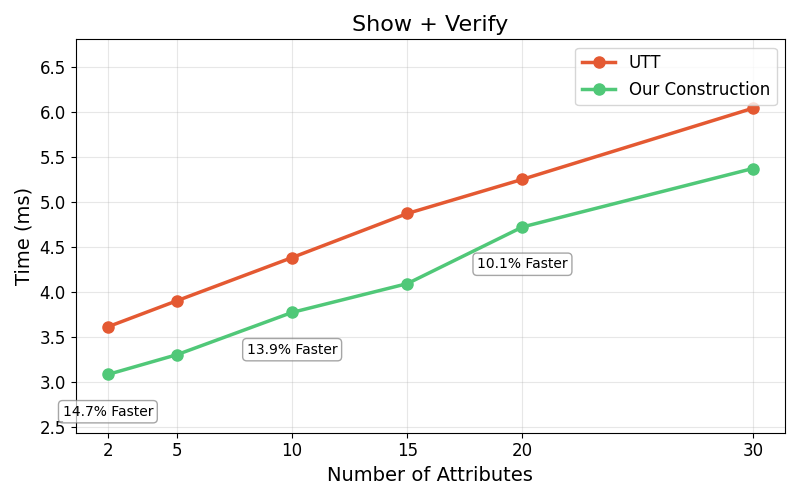
\includegraphics[width=0.95\textwidth]{figures/chap2_show_verify_utt_vs_us.png}
    \end{minipage}

    \vspace{0.05cm}
    
    % Bottom row with 2x2 grid of smaller figures
    \begin{minipage}{0.49\textwidth}
        \centering
        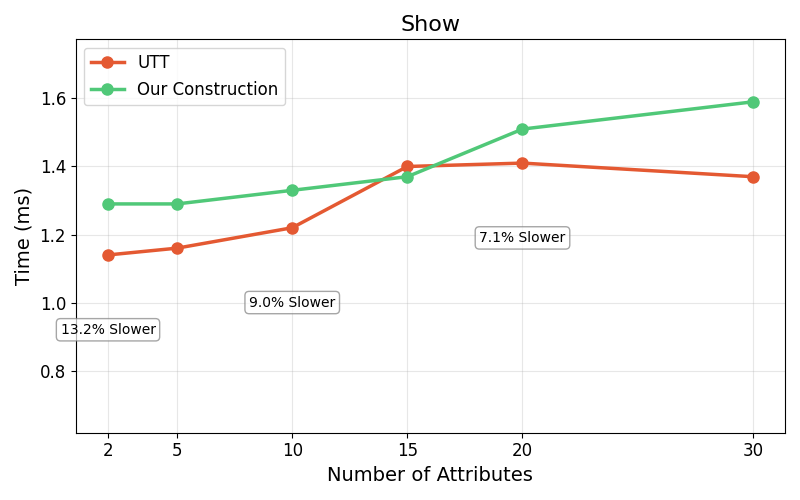
\includegraphics[width=\textwidth]{figures/chap2_show_utt_vs_us.png}
    \end{minipage}
    \hspace{-1em}  % Add negative space to bring plots closer
    \begin{minipage}{0.49\textwidth}
        \centering
        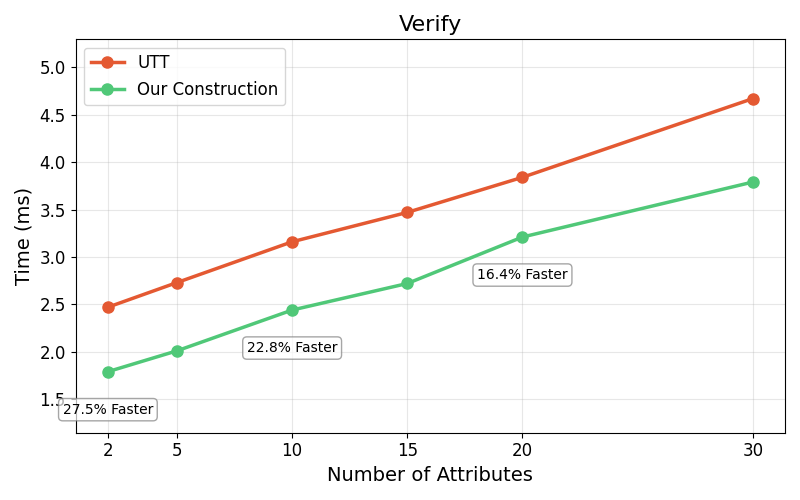
\includegraphics[width=\textwidth]{figures/chap2_verify_utt_vs_us.png}
    \end{minipage}
    
    \caption[Credential Presentation Comparison - My Construction is Fastest]{Credential Presentation Comparison between UTT and my G2 variant - my construction is the fastest by 10 - 15\%}
    \label{fig:show_verify_utt_us}
\end{figure}
\vspace{-0.05cm}
\begin{table}[!htbp]
\centering
\caption{Performance Comparison: UTT and My Construction (time in ms)}
\label{tab:g1-g2-comparison}
\begin{tabular}{l@{\hspace{1em}}r@{\hspace{1.5em}}r@{\hspace{2em}}r@{\hspace{1.5em}}r@{\hspace{2em}}r@{\hspace{1.5em}}r}
\toprule
\textbf{Attributes} & \multicolumn{2}{c@{\hspace{4em}}}{\textbf{Show}} & \multicolumn{2}{c@{\hspace{2.5em}}}{\textbf{Verify}} & \multicolumn{2}{c}{\textbf{Show + Verify}} \\
\cmidrule(lr){2-3} \cmidrule(lr){4-5} \cmidrule(lr){6-7}
 & \textbf{\cite{tomescu_utt_2022}} & \textbf{Mine} & \textbf{\cite{tomescu_utt_2022}} & \textbf{Mine} & \textbf{\cite{tomescu_utt_2022}} & \textbf{Mine} \\
\midrule
2 & 1.14 & 1.29  & 2.47 & 1.79  & 3.61 & 3.08 (14.7\%$\downarrow$) \\
5 & 1.16 & 1.29 & 2.73 & 2.01  & 3.90 & 3.30 (15.4\%$\downarrow$) \\
10 & 1.22 & 1.33  & 3.16 & 2.44  & 4.38 & 3.77 (13.9\%$\downarrow$) \\
15 & 1.40 & 1.37 & 3.47 & 2.72  & 4.87 & 4.09 (16.0\%$\downarrow$) \\
20 & 1.41 & 1.51  & 3.84 & 3.21  & 5.25 & 4.72 (10.1\%$\downarrow$) \\
30 & 1.37 & 1.59 & 4.67 & 3.79  & 6.04 & 5.37 (11.1\%$\downarrow$) \\
\bottomrule
\end{tabular}
\end{table}



















\subsection{Empirically Faster Credential Presentations Compared to Popular Anonymous Credentials. Efficiencies are mainly due to reducing the pairing operation}
I implemented and compared five Anonymous Credential schemes, BBS+ (2006) \cite{hutchison_constant-size_2006}: The original BBS+ signature scheme, BBS+ (2016) \cite{camenisch_anonymous_2016}: An optimized version with proofs in $\G_1$, PS (2016) \cite{sako_short_2016}: The Pointcheval-Sanders scheme, UTT \cite{tomescu_utt_2022}: The UTT variant with signatures in $\mathbb{G}_1$ and my optimized variant with signatures in $\mathbb{G}_2$. I benchmarked the Anonymous Credential algorithms and present the data. Implementations and benchmarks are available for reproduction\footnote{https://github.com/sampolgar/anonymous-credentials} \cite{polgar_anonymous_2025}

\begin{figure}
    \centering
    % First row with two larger figures
    \begin{minipage}{\textwidth}
        \centering
        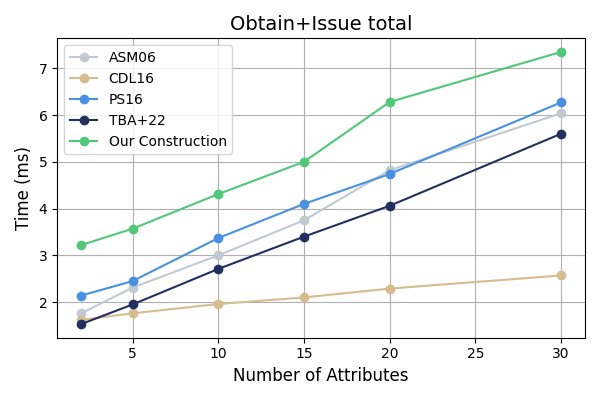
\includegraphics[width=0.75\textwidth]{figures/chap2_anoncreds_obtain_issue.png}
    \end{minipage}
    
    \vspace{0.05cm}
    
    \begin{minipage}{\textwidth}
        \centering
        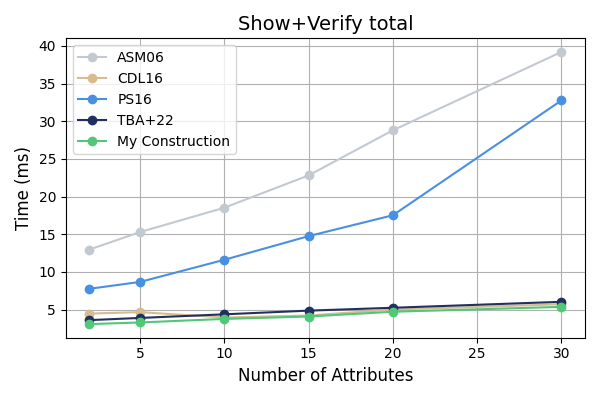
\includegraphics[width=0.75\textwidth]{figures/chap2_anoncreds_show_verify.png}
    \end{minipage}
    
    \vspace{0.05cm}
    
    % Bottom row with 2x2 grid of smaller figures
    \begin{minipage}{0.48\textwidth}
        \centering
        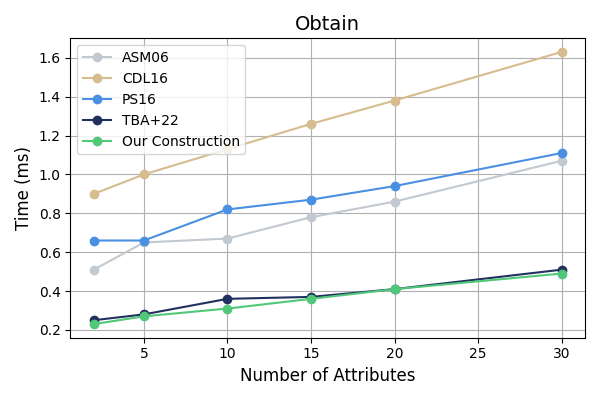
\includegraphics[width=\textwidth]{figures/chap2_anoncreds_obtain.png}
    \end{minipage}
    \hfill
    \begin{minipage}{0.48\textwidth}
        \centering
        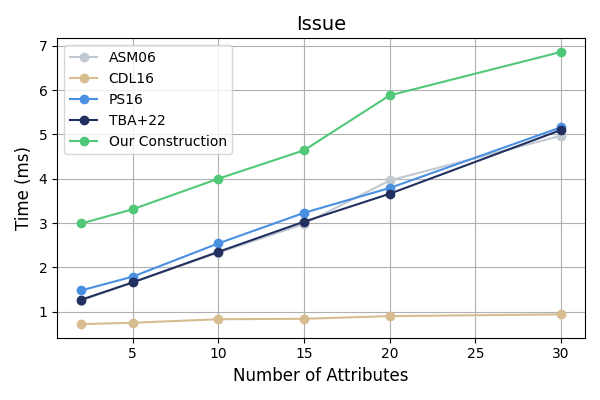
\includegraphics[width=\textwidth]{figures/chap2_anoncreds_issue.png}
    \end{minipage}
    
    \vspace{0.1cm}
    
    \begin{minipage}{0.48\textwidth}
        \centering
        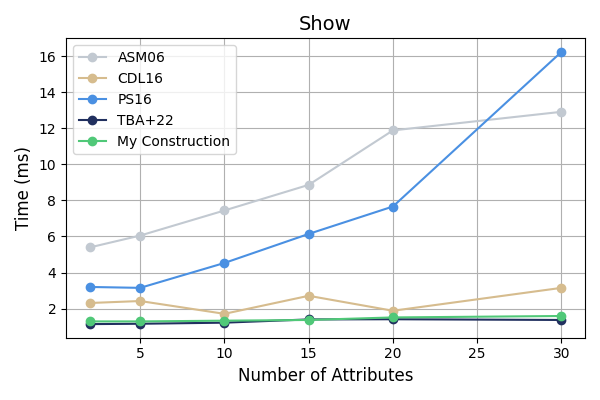
\includegraphics[width=\textwidth]{figures/chap2_anoncreds_show.png}
    \end{minipage}
    \hfill
    \begin{minipage}{0.48\textwidth}
        \centering
        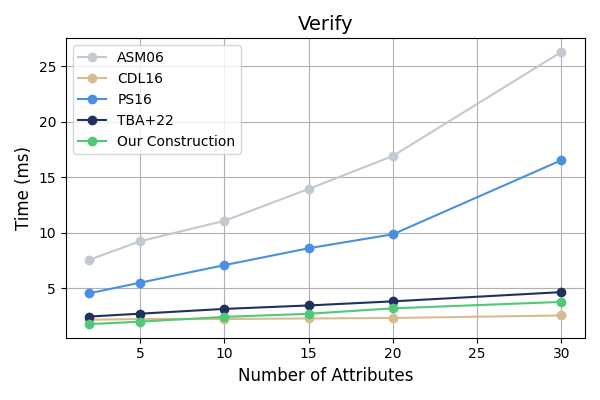
\includegraphics[width=\textwidth]{figures/chap2_anoncreds_verify.png}
    \end{minipage}
    
    \caption{Performance comparison of different operations across varying numbers of attributes}
    \label{fig:anoncreds-performance}
\end{figure}

\begin{table}[htbp]\label{abc-performance-combined-table}
\centering
\caption{Performance of Anonymous Credential Operations (time in ms), $n$ is attribute count}
\begin{tabular}{@{}p{1.2cm}*{5}{>{\centering\arraybackslash}p{1.6cm}}@{}}
\toprule
$n$ & \cite{hutchison_constant-size_2006} & \cite{camenisch_anonymous_2016} & \cite{sako_short_2016} & \cite{tomescu_utt_2022} & My Construction  \ref{subsec:g2_verify_speedup} \\
\midrule
\multicolumn{6}{c}{\textbf{Obtain}}  \\
\midrule
\textbf{2} & 0.51 & 0.90 & 0.66 & 0.25 & \textbf{0.23} \\
\textbf{5} & 0.65 & 1.00 & 0.66 & 0.28 & \textbf{0.27} \\
\textbf{10} & 0.67 & 1.13 & 0.82 & 0.36 & \textbf{0.31} \\
\textbf{15} & 0.78 & 1.26 & 0.87 & 0.37 & \textbf{0.36} \\
\textbf{20} & 0.86 & 1.38 & 0.94 & \textbf{0.41} & \textbf{0.41} \\
\textbf{30} & 1.07 & 1.63 & 1.11 & 0.51 & \textbf{0.49} \\
\midrule
\multicolumn{6}{c}{\textbf{Issue}}  \\
\midrule
\textbf{2} & 1.25 & \textbf{0.72} & 1.48 & 1.27 & 2.99 \\
\textbf{5} & 1.66 & \textbf{0.75} & 1.79 & 1.66 & 3.31 \\
\textbf{10} & 2.33 & \textbf{0.83} & 2.54 & 2.35 & 4.00 \\
\textbf{15} & 2.98 & \textbf{0.84} & 3.23 & 3.03 & 4.64 \\
\textbf{20} & 3.96 & \textbf{0.90} & 3.79 & 3.66 & 5.88 \\
\textbf{30} & 4.97 & \textbf{0.94} & 5.16 & 5.10 & 6.86 \\
\midrule
\multicolumn{6}{c}{\textbf{Show}}  \\
\midrule
\textbf{2} & 5.39 & 2.31 & 3.20 & \textbf{1.14} & 1.29 \\
\textbf{5} & 6.05 & 2.42 & 3.15 & \textbf{1.16} & 1.29 \\
\textbf{10} & 7.44 & 1.71 & 4.53 & \textbf{1.22} & 1.33 \\
\textbf{15} & 8.86 & 2.71 & 6.14 & 1.40 & \textbf{1.37} \\
\textbf{20} & 11.88 & 1.88 & 7.66 & \textbf{1.41} & 1.51 \\
\textbf{30} & 12.91 & 3.15 & 16.23 & \textbf{1.37} & 1.59 \\
\midrule
\multicolumn{6}{c}{\textbf{Verify}}  \\
\midrule
\textbf{2} & 7.59 & 2.18 & 4.57 & 2.47 & \textbf{1.79} \\
\textbf{5} & 9.25 & 2.25 & 5.52 & 2.73 & \textbf{2.01} \\
\textbf{10} & 11.09 & \textbf{2.25} & 7.10 & 3.16 & 2.44 \\
\textbf{15} & 13.96 & \textbf{2.30} & 8.62 & 3.47 & 2.72 \\
\textbf{20} & 16.93 & \textbf{2.34} & 9.88 & 3.84 & 3.21 \\
\textbf{30} & 26.30 & \textbf{2.57} & 16.55 & 4.67 & 3.79 \\
\midrule
\multicolumn{6}{c}{\textbf{Issuing Phase Total (Obtain + Issue)}}  \\
\midrule
\textbf{2} & 1.76 & 1.62 & 2.14 & \textbf{1.53} & 3.22 \\
\textbf{5} & 2.31 & \textbf{1.76} & 2.45 & 1.95 & 3.57 \\
\textbf{10} & 3.00 & \textbf{1.96} & 3.37 & 2.71 & 4.31 \\
\textbf{15} & 3.75 & \textbf{2.10} & 4.10 & 3.40 & 5.00 \\
\textbf{20} & 4.82 & \textbf{2.29} & 4.74 & 4.06 & 6.28 \\
\textbf{30} & 6.04 & \textbf{2.57} & 6.27 & 5.60 & 7.35 \\
\midrule
\multicolumn{6}{c}{\textbf{Showing Phase Total (Show + Verify)}}  \\
\midrule
\textbf{2} & 12.98 & 4.48 & 7.77 & 3.61 & \textbf{3.08} \\
\textbf{5} & 15.30 & 4.67 & 8.68 & 3.90 & \textbf{3.30} \\
\textbf{10} & 18.53 & 3.96 & 11.62 & 4.38 & \textbf{3.77} \\
\textbf{15} & 22.82 & 4.22 & 14.76 & 4.87 & \textbf{4.09} \\
\textbf{20} & 28.81 & 5.01 & 17.53 & 5.25 & \textbf{4.72} \\
\textbf{30} & 39.21 & 5.72 & 32.77 & 6.04 & \textbf{5.37} \\
\bottomrule
\end{tabular}
\end{table}

\subsubsection{Key Findings}
\begin{enumerate}
    \item \textbf{Optimized}: My PS-UTT G2 variant achieves the best Show+Verify performance (10-16\% faster than PS-UTT G1 and up to 83\% faster than BBS+ 2006), optimizing the operation that occurs most frequently in practice. While the Issue operation is more costly, credentials are issued once but verified many times.
    
    \item \textbf{Evolution of Efficiency}: The original constructions \cite{hutchison_constant-size_2006, sako_short_2016} required proof of knowledge for $\mathbb{G}_T$ points, resulting in slower operations. Later optimizations \cite{camenisch_anonymous_2016, tomescu_utt_2022} shifted proof of knowledge work to $\G_1$ reducing Show+Verify time by up to 6x. 
    
    \item \textbf{Favorable Scaling Properties}: While all schemes exhibit approximately linear scaling with attribute count, My PS-UTT G2 is the most efficient.
\end{enumerate}




\section{Summary and Future Work}
Investigating concrete benchmarks for different proof systems is a practically useful avenue for exploration. Based on the literature and our experiments, $\Sigma-$protocols are extremely expressive and efficient though are not compatible with many signature and algebraic constructions, such as hash functions and group elements. 
Furthermore, detailed comparisons should be made between these constructions and zkSNARKS \cite{ben-sasson_snarks_2013}, particularly of the STARK \cite{ben-sasson_stark_2020} variety, which are secure against quantum adversaries. Doing so may significantly change the architecture of Anonymous Credentials as is done in \cite{rosenberg_zk-creds_2022}.






























% \begin{figure}
%     \centering
% \begin{pcvstack}[boxed]
%         \procedure[linenumbering]{$\mathrm{Sim}^{\mathsf{\UNF}}_{\MIMCABC, \adv}(\lambda)$}{%
%             \AdvB \text{ Setup Simulation  } \\
%             \vk \gets \text{Challenge from } \EUFCMA \text{ game from $\RS$} \\
%             \ck \gets \text{Challenge from } \POSBINDING \text{ game from $\CM$} \\
%             \AdvB \text{ Embeds $\vk, \ck$ into $\MIMCABC$ public params $\pp$ and issuer keys $\{\opk_j\}$} \\
%             \text{Simulating $\mathrm{Game}^{\mathsf{UNF}_{\MIMCABC}}$ setup for $\AdvA$} 
%             \\
%             \AdvB \text{ uses real $\OHU, \OCU$ and simulates $\OOBTAIN, \OSHOW$} \\
%             \AdvA \text{ outputs forgery } \{ \cred_k'^*, \phi^*, \pi^* \} \\
%             \AdvB \text{ processes the forgery to break the assumption}
%         }
%         \procedure[]{$\AdvB$ Simulates $\OOBTAIN(i, j, \vec{m})$}{%
%             \pcif i \notin \HU, \pcreturn \bot \quad \greyt{// Only honest users can obtain credentials} \\
%             \t \usk \gets \mathbb{Z}_p \quad \greyt{// Generate fresh randomness for commitment} \\
%             \t \cm \gets \CMCom(\vec{m}; \usk) \quad \greyt{// Commitment to attributes} \\
%             \t \pcif j \neq j^*, \\
%             \t \t \sigma \gets \RSSign(\osk_j, \cm) \quad \greyt{// Sign using known issuer key} \\
%             \t \pcelse \quad \greyt{// Case: } j = j^* \\
%             \t \t \sigma \gets \OEUFCMA(\cm) \quad \greyt{// Query EUF-CMA oracle for signature} \\
%             \t \cred \gets (\sigma, \cm) \quad  \\
%             \t \CRED_j \gets \CRED_j \cup \{(\cred, \cm, \vec{m}, \usk, i)\} \\
%             \t \OWNR[\cred] \gets i \\
%             \pcreturn \cred
%         }
%         \procedure[]{$\AdvB$ Simulates $\OSHOW(i, \phi)$}{%
%             \pcif i \notin \HU, \pcreturn \bot \quad \greyt{// Only honest users can show proofs} \\
%             \t \text{Let } \creds_i \text{ be the credentials of user } i \text{ in } \HU \\
%             \t \pcif \phi(\text{attributes in } \creds_i) = 0, \pcreturn \bot \quad \greyt{// Check policy satisfaction} \\
%             \t \pi \gets \text{ZKSim}(\phi, \{ \cred_k' \}, \{ \cm_k' \}, \text{ Simulate proof without witness})\\
%             \SHOW \gets \SHOW \cup (i, \phi, \pi) \\
%             \pcreturn \pi
%         }
%     \end{pcvstack}
%     \caption{Simulated Oracles}
    
% \end{figure}

